\documentclass[11pt]{article}
\usepackage[a3paper,landscape,margin=15mm]{geometry}

\usepackage{fontspec}
\setmainfont{Nimbus Roman}
\setsansfont{Nimbus Sans}
\setmonofont{Nimbus Mono PS}
\usepackage[authoryear]{natbib}
\usepackage{amsmath,amssymb,graphicx,booktabs,array,xcolor,caption,tikz,longtable}
\usetikzlibrary{positioning,fit,arrows.meta}
\usepackage{microtype}
\microtypesetup{expansion=false}
\usepackage{url}
\setlength{\emergencystretch}{3em}
\setlength{\parindent}{0pt}
\setlength{\parskip}{4pt}
\newcommand{\ibar}{\bar{y}}
\newcommand{\sbar}{\bar{s}}
\newcommand{\Exp}{\mathrm{Exp}}
\newcommand{\Full}{\textnormal{Full}}
\newcommand{\TS}{\textnormal{TwoScale}}
\newcommand{\ind}{\mathbf{1}}
\newcommand{\eW}{e_W}
\newcommand{\qed}{\hfill\(\square\)}
\newsavebox{\mathbox}
\newcommand{\fitmath}[1]{%
  \sbox{\mathbox}{$\displaystyle #1$}%
  \ifdim\wd\mathbox>\linewidth
    \resizebox{\linewidth}{!}{\usebox{\mathbox}}%
  \else\usebox{\mathbox}\fi}

\begin{document}
\begin{center}\Large Розділи 1--5: простіша українська редакція\end{center}
Відповідні фрагменти вирівняно поруч. Нумерація розділів, формул і посилань відповідає вихідній статті.
\setlength{\tabcolsep}{6mm}
\begin{longtable}{@{}p{0.475\textwidth}|p{0.475\textwidth}@{}}
\Large\textbf{До} & \Large\textbf{Після}\\\hline\endhead
\begin{minipage}[t]{\linewidth}
\section*{1. Вступ}

\end{minipage} &
\begin{minipage}[t]{\linewidth}
\section*{1. Вступ}

\end{minipage} \\*[5mm]
\begin{minipage}[t]{\linewidth}
Епідемія поширюється на кількох рівнях. Усередині спільноти зараження може залежати від конкретних контактів між людьми \citep{keeling2005,pastorsatorras2015,kiss2017}. Для зв'язків між спільнотами дані часто менш докладні: наприклад, відома лише кількість пасажирів, обсяг поїздок на роботу або загальна вага зв'язку між двома місцями \citep{balcan2009,barbosa2018human}. Тому потрібна модель, яка поєднує докладну контактну мережу всередині кожної спільноти із загальними даними про зв'язки між спільнотами.
\end{minipage} &
\begin{minipage}[t]{\linewidth}
Інфекція поширюється як усередині спільнот, так і між ними. Усередині спільноти важливо, хто саме з ким контактує \citep{keeling2005,pastorsatorras2015,kiss2017}. Про зв'язки між спільнотами часто відомо менше: наприклад, лише кількість пасажирів або поїздок на роботу \citep{balcan2009,barbosa2018human}. Ми досліджуємо модель, яка зберігає окремі контакти всередині спільнот, а зв'язки між ними описує загальними вагами.
\end{minipage} \\[5mm]
\begin{minipage}[t]{\linewidth}
Така ситуація виникає на практиці. Локальну контактну мережу можна спостерігати, відновлювати або генерувати за відомими характеристиками, зокрема кластеризацією та середньою довжиною найкоротших шляхів \citep{eubank2004,danon2011}. Натомість зв'язки між спільнотами можуть бути відомі лише з транспортних, міграційних даних, даних про поїздки на роботу чи даних мобільних операторів \citep{barbosa2018human,chang2021}. Вони дають загальну силу зв'язку, але не визначають людей, через яких інфекція може перейти між спільнотами. Отже, ми можемо знати вагу зв'язку, не знаючи конкретних вузлів-мостів та їхнього стану.
\end{minipage} &
\begin{minipage}[t]{\linewidth}
Контактні мережі можна будувати за даними про населення, його переміщення та контакти \citep{eubank2004,danon2011}. Зв'язки між спільнотами можна оцінювати за транспортними й міграційними даними або даними мобільних операторів \citep{barbosa2018human,chang2021}. Такі дані показують, наскільки сильно пов'язані дві спільноти, але не завжди вказують конкретних людей, через яких може перейти інфекція. Вузли, що мають контакти з іншою спільнотою, далі називаємо вузлами-мостами.
\end{minipage} \\[5mm]
\begin{minipage}[t]{\linewidth}
Якщо відомі всі контакти, епідемію можна описати неперервним марковським ланцюгом (CTMC) і точно моделювати методом Gillespie \citep{gillespie1977exact,gibson2000}. Є також ефективні методи для часових, великих і розріджених мереж \citep{vestergaard2015,kuryliak2025simulating}. Проте їм усе одно потрібні конкретні контакти, здатні передавати інфекцію. Метапопуляційні моделі використовують загальні потоки між спільнотами, але зазвичай замінюють і докладну локальну мережу кількостями людей у різних станах \citep{colizza2007reaction,colizza2008,balcan2010modeling,ajelli2010}. Наша задача лежить між цими двома випадками: зберегти випадкове поширення між окремими вузлами всередині спільнот, використовуючи лише загальні дані для зв'язків між ними.
\end{minipage} &
\begin{minipage}[t]{\linewidth}
Якщо відомі всі контакти, можна моделювати випадкові зараження методом Gillespie. Він точно відтворює заданий неперервний марковський ланцюг (CTMC) \citep{gillespie1977exact,gibson2000}. Існують також ефективні алгоритми для мереж зі змінними в часі контактами та для мережевого моделювання епідемій \citep{vestergaard2015,kuryliak2025simulating}. Їм потрібні конкретні контакти, через які передається інфекція. Метапопуляційні моделі натомість описують спільноти кількостями людей у різних станах і зв'язують їх загальними потоками \citep{colizza2007reaction,colizza2008,balcan2010modeling,ajelli2010}. Ми поєднуємо ці підходи: моделюємо окремі вузли всередині спільнот і використовуємо загальні ваги для передавання між ними.
\end{minipage} \\[5mm]
\begin{minipage}[t]{\linewidth}
Ідею двомасштабного симулятор представлено в попередній конференційній роботі \citep{kuryliak2025towards}. Для кожної спільноти він запускає окремий локальний симулятор. Макрорівень використовує поточні стани спільнот і ваги зв'язків, щоб генерувати зараження, які надходять з іншої спільноти. У цій статті ми докладно описуємо метод і досліджуємо його похибку. Зокрема, з'ясовуємо, що втрачається, коли справжні міжспільнотні ребра та їхні кінцеві вузли замінено загальною вагою зв'язку, а імпортоване зараження потрапляє на випадково вибраний сприйнятливий вузол.
\end{minipage} &
\begin{minipage}[t]{\linewidth}
Ідею двомасштабного симулятора представлено в попередній конференційній роботі \citep{kuryliak2025towards}. Кожна спільнота має свій локальний симулятор. Спільний планувальник, який називаємо макрорівнем, визначає зараження між спільнотами за їхніми поточними станами та вагами зв'язків. Зараження, що надходить з іншої спільноти, називаємо імпортом інфекції. У цій статті описуємо метод і досліджуємо його похибку: що змінюється, коли замість справжніх міжспільнотних контактів відома лише їхня загальна вага, а імпорт потрапляє на випадково вибраний сприйнятливий вузол?
\end{minipage} \\[5mm]
\begin{minipage}[t]{\linewidth}
Головне питання: коли такого агрегованого зв'язку достатньо для відтворення потрібної нам характеристики повномережевого CTMC? Ми досліджуємо часи прибуття інфекції, їхні розподіли та можливість передавання через справжні контакти. Близькі часи прибуття ще не гарантують фізично можливого передавання: агрегована модель може заразити іншу спільноту до того, як заразиться будь-який справжній вузол-міст у спільноті-джерелі. У контрольованих експериментах ми знаємо повну контактну мережу й використовуємо її як еталон. Двомасштабний симулятор отримує лише локальні мережі та загальні ваги зв'язків. Це перевірка методу, а не калібрування моделі конкретної епідемії.
\end{minipage} &
\begin{minipage}[t]{\linewidth}
Головне питання: коли цього спрощення достатньо, щоб правильно оцінити час поширення інфекції? Ми порівнюємо часи її першого прибуття до спільнот і розподіли цих часів за багатьма запусками. Також перевіряємо, чи могло зараження відбутися через справжні контакти. Близькі часи ще не гарантують можливого шляху передавання: двомасштабна модель може заразити іншу спільноту, поки всі справжні вузли-мости в спільноті-джерелі ще сприйнятливі. Для перевірки ми використовуємо синтетичні мережі, у яких знаємо всі контакти. Повний Gillespie отримує всю мережу, а двомасштабний метод --- лише локальні мережі та загальні ваги міжспільнотних зв'язків.
\end{minipage} \\[5mm]
\begin{minipage}[t]{\linewidth}
Стаття має чотири основні результати.
\begin{enumerate}
\item Ми повністю описуємо двомасштабний симулятор, зокрема синхронізацію локальних симуляторів з глобальним з через фіксовані часові інтервали (Розділ~3, Алгоритм~1).
\item Ми показуємо, що саме моделює ідеальний метод із неперервним часом. Він точний для \emph{сурогатної мережі}: справжні міжспільнотні ребра замінено слабкими зв'язками між усіма парами вузлів зі збереженням загальної ваги (Твердження~1). Далі ми визначаємо джерела похибки та аналізуємо один експорт інфекції (Твердження~2).
\item Ми порівнюємо метод із повномережевим моделюванням Gillespie для одиничних експортів і ланцюгів спільнот. Перестановочні перевірки показують, які відмінності можуть виникнути лише через скінченну кількість запусків (Розділи~5 і~6).
\item Ми пропонуємо емпіричний показник точності для наших тестів. Він порівнює розкид часів зараження всередині спільноти з типовим часом передавання через одне міжспільнотне ребро (Розділ~6.6).
\end{enumerate}
\end{minipage} &
\begin{minipage}[t]{\linewidth}
Стаття має чотири основні результати.
\begin{enumerate}
\item Описуємо, як працює симулятор: кожна спільнота моделюється окремо, а спільний планувальник визначає зараження між ними. Пояснюємо, як він узгоджує локальні симулятори на часових інтервалах фіксованої довжини (Розділ~3, Алгоритм~1).
\item Показуємо, яку мережу метод моделює точно, якщо визначати час кожної події без наближення часовою сіткою. Це \emph{сурогатна мережа}: справжні контакти між двома спільнотами замінено слабкими зв'язками між усіма парами їхніх вузлів зі збереженням загальної ваги (Твердження~1). Пояснюємо джерела похибки цієї заміни. Для одного передавання назовні доводимо, що за випадкового рівномірного розміщення мостів такий метод схильний передавати інфекцію раніше за повний Gillespie; точний зміст цього порівняння наведено в Твердженні~2.
\item Порівнюємо метод із повним Gillespie для одного передавання інфекції назовні та для ланцюгів спільнот. У наших тестах за швидкого поширення всередині спільнот розподіли часу прибуття зазвичай близькі. За повільнішого внутрішнього поширення двомасштабний метод систематично дає раніше прибуття. Випадкове переставляння міток методів у результатах запусків допомагає оцінити, чи можна пояснити відмінності скінченною кількістю запусків (Розділи~5 і~6).
\item Пропонуємо показник, який допомагає пояснити точність у наших тестах. Він порівнює розкид часів зараження всередині спільноти із середнім часом передавання через одне міжспільнотне ребро. За малих значень розподіли часу прибуття зазвичай узгоджуються; за більших метод дає раніше прибуття. Це спостереження для досліджених мереж, а не загальний закон похибки (Розділ~6.6).
\end{enumerate}
\end{minipage} \\[5mm]
\begin{minipage}[t]{\linewidth}
Ми розглядаємо динаміку «сприйнятливий--інфікований» (SI) на статичних синтетичних мережах і використовуємо один фіксований крок синхронізації. Розділ~2 пояснює зв'язок із попередніми методами. Розділ~3 описує симулятор. У Розділі~4 пояснено, яку інформацію агрегований зв'язок зберігає та втрачає. Розділи~5 і~6 містять експерименти та результати. У Розділі~7 обговорено застосування, обчислювальні витрати й обмеження.
\end{minipage} &
\begin{minipage}[t]{\linewidth}
У всіх експериментах вузол після зараження залишається інфікованим: це модель «сприйнятливий--інфікований» (SI). Мережі статичні й синтетичні, а крок синхронізації фіксований. Далі описуємо попередні праці (Розділ~2), метод (Розділ~3) та інформацію, яку він зберігає і втрачає (Розділ~4). Експерименти й результати наведено в Розділах~5 і~6, а застосування та обмеження --- у Розділі~7.
\end{minipage} \\[5mm]
\begin{minipage}[t]{\linewidth}
\section*{2. Пов'язані праці}

\end{minipage} &
\begin{minipage}[t]{\linewidth}
\section*{2. Пов'язані праці}

\end{minipage} \\*[5mm]
\begin{minipage}[t]{\linewidth}
\paragraph{Моделювання випадкових подій.}
Прямий метод Gillespie вибирає наступну подію та її час за поточними інтенсивностями подій \citep{gillespie1977exact}. Метод наступної реакції підтримує окремий годинник для кожної можливої події \citep{gibson2000}. Обидва методи точні для CTMC, який вони моделюють. Якщо інтенсивність змінюється з часом, її можна накопичувати до досягнення випадкового порога \citep{ethier1986}. \citet{anderson2007} використав цю ідею для систем зі змінними інтенсивностями та затримками. Наш макрогодинник працює за тією самою ідеєю, але його інтенсивність змінюється разом зі станами локальних епідемій. Мережеві симулятори можуть зменшувати обсяг роботи, оновлюючи лише інтенсивності, на які вплинула остання подія \citep{vestergaard2015,kuryliak2025simulating}. Наші локальні симулятори використовують реалізацію з \citet{kuryliak2025simulating}.
\end{minipage} &
\begin{minipage}[t]{\linewidth}
\paragraph{Моделювання випадкових подій.}
Прямий метод Gillespie визначає час наступної події та вибирає її за поточними інтенсивностями --- величинами, що задають частоту подій \citep{gillespie1977exact}. Метод наступної реакції веде окремий годинник для кожної можливої події \citep{gibson2000}. Обидва точно моделюють заданий CTMC. Якщо інтенсивність змінюється, час події можна визначати, накопичуючи її до випадкового порога \citep{ethier1986}. \citet{anderson2007} застосував цю ідею до систем зі змінними інтенсивностями та затримками. Так само працює наш годинник міжспільнотних заражень. Для ефективного мережевого моделювання використовують, зокрема, часовий алгоритм Gillespie та оновлення лише тих інтенсивностей, які змінила остання подія \citep{vestergaard2015,kuryliak2025simulating}. Наші локальні симулятори використовують реалізацію з \citet{kuryliak2025simulating}.
\end{minipage} \\[5mm]
\begin{minipage}[t]{\linewidth}
Деякі багатомасштабні методи прискорюють моделювання хімічних реакцій, наближено описуючи реакції, що відбуваються значно частіше за інші \citep{haseltine2002,cao2005slow}. Наш метод прибирає іншу інформацію. Він зберігає локальні зараження, але не знає, які саме міжспільнотні ребра зараз здатні передавати інфекцію. Попри цю відмінність, співвідношення швидкостей локального поширення та міжспільнотного передавання допомагає пояснити похибку.
\end{minipage} &
\begin{minipage}[t]{\linewidth}
Багатомасштабні методи для хімічних реакцій можуть наближено описувати швидкі реакції, щоб прискорити моделювання \citep{haseltine2002,cao2005slow}. Наше спрощення стосується контактів: локальні зараження моделюються окремо, але конкретні міжспільнотні ребра невідомі. Співвідношення часу поширення всередині спільноти й часу передавання між спільнотами допомагає пояснити наслідки цього спрощення.
\end{minipage} \\[5mm]
\begin{minipage}[t]{\linewidth}
\paragraph{Моделі з кількома спільнотами.}
Метапопуляційні моделі описують кожну підпопуляцію кількостями людей у різних станах і зв'язують підпопуляції потоками мобільності. Їх використовували для дослідження глобального поширення та умов проникнення інфекції \citep{colizza2007reaction,colizza2008,balcan2009,balcan2010modeling}. Докладні дані мобільності також можна поєднувати з локальними моделями передавання \citep{chang2021}. Агентні моделі, своєю чергою, представляють окремих людей у всій системі \citep{eubank2004,kerr2021}. \citet{ajelli2010} порівняли ці два підходи. Досліджуваний тут метод зберігає окремі вузли та контакти всередині спільноти, але замінює невідомі індивідуальні контакти між спільнотами одним агрегованим стохастичним зв'язком.
\end{minipage} &
\begin{minipage}[t]{\linewidth}
\paragraph{Моделі з кількома спільнотами.}
Метапопуляційні моделі рахують людей у різних станах у кожній спільноті й описують переміщення між спільнотами. Так досліджують глобальне поширення та умови проникнення інфекції \citep{colizza2007reaction,colizza2008,balcan2009,balcan2010modeling}. Дані про переміщення також поєднують із локальними моделями передавання \citep{chang2021}. Агентні моделі описують окремих людей у всій системі \citep{eubank2004,kerr2021}. \citet{ajelli2010} порівняли ці підходи. Наш метод зберігає окремі вузли та контакти всередині спільнот, а зараження між ними визначає за загальними вагами зв'язків і поточними кількостями вузлів у різних станах.
\end{minipage} \\[5mm]
\begin{minipage}[t]{\linewidth}
\paragraph{Два рівні перемішування та спільне моделювання.}
Деякі епідемічні моделі поєднують контакти в малих локальних групах із рівномірним перемішуванням на ширшому рівні \citep{ball1997}. Наша сурогатна мережа має подібну ідею, але рівномірне перемішування діє лише між зв'язаними парами спільнот, а його силу визначає загальна вага зв'язку.
\end{minipage} &
\begin{minipage}[t]{\linewidth}
\paragraph{Два рівні перемішування та спільне моделювання.}
Деякі епідемічні моделі враховують окремі контакти в малих групах, а на ширшому рівні припускають рівномірне перемішування \citep{ball1997}. Подібне припущення має наша сурогатна мережа: між двома зв'язаними спільнотами загальну вагу рівномірно розподілено між усіма парами вузлів.
\end{minipage} \\[5mm]
\begin{minipage}[t]{\linewidth}
Реалізація також має риси спільного моделювання (co-simulation). У ньому окремі симулятори підсистем рухаються вперед за спільною часовою сіткою та обмінюються обмеженим набором даних \citep{gomes2018cosim}. У нас цими підсистемами є локальні симулятори спільнот. Вони передають макрорівню кількості інфікованих і сприйнятливих вузлів. Макрорівень використовує ці дані, щоб згенерувати час міжспільнотного зараження та вибрати спільноту-одержувача й цільовий вузол. Отже, локальні симулятори можуть залишатися «чорними скриньками» для планувальника. У цій реалізації дані, якими вони обмінюються, використовуються для створення випадкових подій зараження.
\end{minipage} &
\begin{minipage}[t]{\linewidth}
Метод також пов'язаний зі спільним моделюванням (co-simulation): окремі симулятори працюють за узгодженими часовими інтервалами й обмінюються даними \citep{gomes2018cosim}. У нас кожен локальний симулятор повідомляє кількості інфікованих і сприйнятливих вузлів. Планувальник використовує їх для визначення часу міжспільнотного зараження та вибору його цілі. Йому не потрібно знати всі внутрішні кроки локальних симуляторів.
\end{minipage} \\[5mm]
\begin{minipage}[t]{\linewidth}
\section*{3. Метод двомасштабного моделювання}

\end{minipage} &
\begin{minipage}[t]{\linewidth}
\section*{3. Метод двомасштабного моделювання}

\end{minipage} \\*[5mm]
\begin{minipage}[t]{\linewidth}
В експериментах використано одну реалізацію двомасштабного симулятора, яка узгоджує спільноти за часовою сіткою. Щоб зрозуміти її похибку, ми також розглядаємо процес із тими самими інтенсивностями, але з точним визначенням часу кожної події. Цей теоретичний опис називаємо \emph{ідеальним процесом}. Він дає змогу відокремити похибку заміни мережі від додаткової похибки часової сітки. Ідеальний процес точний для сурогатної мережі, визначеної далі; це не означає точності для початкової фізичної мережі. Нижче пояснимо еталонну модель, доступні дані та кроки реалізованого симулятора.
\end{minipage} &
\begin{minipage}[t]{\linewidth}
Усі експерименти використовують одну реалізацію двомасштабного симулятора. Вона узгоджує локальні симулятори на часових інтервалах фіксованої довжини та наближено визначає час зараження між спільнотами. Для пояснення похибки також розглядаємо теоретичну версію з точним часом кожної події. Далі називаємо її \emph{ідеальним процесом}. Це двомасштабний метод без чисельної похибки часової сітки. Він усе ще використовує усереднені зв'язки між спільнотами, тому точно моделює сурогатну мережу, а загалом не початкову мережу зі справжніми контактами. Нижче описуємо обидві мережі та роботу симулятора.
\end{minipage} \\[5mm]
\begin{minipage}[t]{\linewidth}
\subsection*{3.1. Повномережева еталонна модель}

\end{minipage} &
\begin{minipage}[t]{\linewidth}
\subsection*{3.1. Повномережева еталонна модель}

\end{minipage} \\*[5mm]
\begin{minipage}[t]{\linewidth}
Нехай $G=(V,E)$ --- контактна мережа. Її вузли поділено на $M$ спільнот, які не перетинаються:
\begin{equation*}V=V_1\cup V_2\cup\cdots\cup V_M,
\qquad N_i=|V_i|.\tag{1}
\end{equation*}
Тут $V_i$ --- множина вузлів спільноти $i$, а $N_i$ --- кількість її вузлів. Позначаємо через $E_{ii}$ контакти всередині спільноти $i$, а через $E_{ij}$ --- контакти від вузлів спільноти $i$ до вузлів спільноти $j$. Контакт представляємо як напрямлений канал передавання. Тому ненапрямлений контакт дає два канали --- по одному в кожному напрямку.
\end{minipage} &
\begin{minipage}[t]{\linewidth}
Нехай $G=(V,E)$ --- контактна мережа. Її вузли поділено на $M$ спільнот, які не перетинаються:
\begin{equation*}V=V_1\cup V_2\cup\cdots\cup V_M,
\qquad N_i=|V_i|.\tag{1}
\end{equation*}
Тут $V_i$ --- множина вузлів спільноти $i$, а $N_i$ --- кількість її вузлів. Позначаємо через $E_{ii}$ контакти всередині спільноти $i$, а через $E_{ij}$ --- контакти від вузлів спільноти $i$ до вузлів спільноти $j$. Контакт представляємо як напрямлений канал передавання. Тому ненапрямлений контакт дає два канали --- по одному в кожному напрямку.
\end{minipage} \\[5mm]
\begin{minipage}[t]{\linewidth}
Кожен вузол є сприйнятливим ($S$), інфікованим ($I$) або видаленим ($R$). Повний стан мережі в час $t$ позначаємо $X(t)$, а стан спільноти $i$ --- $X_i(t)$. Множини сприйнятливих та інфікованих вузлів цієї спільноти позначаємо $S_i(t)$ та $I_i(t)$. Їхні кількості --- $s_i(t)$ та $y_i(t)$, а частки --- $\sbar_i(t)=s_i(t)/N_i$ та $\ibar_i(t)=y_i(t)/N_i$. Далі $x$ означає конкретний стан мережі; $x^{v:I}$ --- той самий стан після зараження вузла $v$, а $x^{u:R}$ --- після видалення вузла $u$.
\end{minipage} &
\begin{minipage}[t]{\linewidth}
Кожен вузол є сприйнятливим ($S$), інфікованим ($I$) або видаленим ($R$). Повний стан мережі в час $t$ позначаємо $X(t)$, а стан спільноти $i$ --- $X_i(t)$. Множини сприйнятливих та інфікованих вузлів цієї спільноти позначаємо $S_i(t)$ та $I_i(t)$. Їхні кількості --- $s_i(t)$ та $y_i(t)$, а частки --- $\sbar_i(t)=s_i(t)/N_i$ та $\ibar_i(t)=y_i(t)/N_i$. Далі $x$ означає конкретний стан мережі; $x^{v:I}$ --- той самий стан після зараження вузла $v$, а $x^{u:R}$ --- після видалення вузла $u$.
\end{minipage} \\[5mm]
\begin{minipage}[t]{\linewidth}
Повна модель має два прості правила. Сприйнятливий вузол $v$ отримує інфекцію від кожного інфікованого сусіда $u$ з інтенсивністю $\beta_{uv}$. Інфікований вузол видаляється з інтенсивністю $\gamma$. Для вузлів у відповідних станах:
\begin{equation*}q_v(x)=\sum_{\substack{u:(u,v)\in E\\x_u=I}}\beta_{uv}
\quad (x_v=S),
\qquad r_u(x)=\gamma\quad (x_u=I).\tag{2}
\end{equation*}
Тут $q_v$ --- сумарна інтенсивність зараження вузла $v$, а $r_u$ --- інтенсивність видалення вузла $u$. Для несприйнятливого вузла $q_v=0$; для неінфікованого вузла $r_u=0$. Інтенсивність визначає частоту події: наприклад, за сталої інтенсивності $q$ середній час очікування дорівнює $1/q$. Ці правила також визначають генератор CTMC $\mathcal{L}_G$, використаний далі; ця назва не додає нових правил епідемії. Для міжспільнотного каналу записуємо $\beta_{uv}=\beta_{\mathrm{out}}w_{uv}$, де $w_{uv}$ --- вага контакту. Точне моделювання цих повномережевих інтенсивностей позначаємо \Full{}. Усі експерименти в статті мають динаміку SI, тобто $\gamma=0$.
\end{minipage} &
\begin{minipage}[t]{\linewidth}
Повна модель має два прості правила. Сприйнятливий вузол $v$ отримує інфекцію від кожного інфікованого сусіда $u$ з інтенсивністю $\beta_{uv}$. Інфікований вузол видаляється з інтенсивністю $\gamma$. Для вузлів у відповідних станах:
\begin{equation*}q_v(x)=\sum_{\substack{u:(u,v)\in E\\x_u=I}}\beta_{uv}
\quad (x_v=S),
\qquad r_u(x)=\gamma\quad (x_u=I).\tag{2}
\end{equation*}
Тут $q_v$ --- сумарна інтенсивність зараження вузла $v$, а $r_u$ --- інтенсивність видалення вузла $u$. Для несприйнятливого вузла $q_v=0$; для неінфікованого вузла $r_u=0$. Інтенсивність визначає частоту події: наприклад, за сталої інтенсивності $q$ середній час очікування дорівнює $1/q$. Ці правила також визначають генератор CTMC $\mathcal{L}_G$, використаний далі; ця назва не додає нових правил епідемії. Для міжспільнотного каналу записуємо $\beta_{uv}=\beta_{\mathrm{out}}w_{uv}$, де $w_{uv}$ --- вага контакту. Точне моделювання цих повномережевих інтенсивностей позначаємо \Full{}. Усі експерименти в статті мають динаміку SI, тобто $\gamma=0$.
\end{minipage} \\[5mm]
\begin{minipage}[t]{\linewidth}
\subsection*{3.2. Агрегований інтерфейс}

\end{minipage} &
\begin{minipage}[t]{\linewidth}
\subsection*{3.2. Агрегований інтерфейс}

\end{minipage} \\*[5mm]
\begin{minipage}[t]{\linewidth}
Двомасштабний симулятор \TS{} знає кожен локальний граф $G_i=(V_i,E_{ii})$ та його інтенсивності. Він не знає конкретних міжспільнотних каналів у $E_{ij}$. Для кожної напрямленої пари спільнот йому відома лише загальна вага:
\begin{equation*}W_{ij}=\sum_{(u,v)\in E_{ij}}w_{uv},\qquad i\neq j.\tag{3}
\end{equation*}
Якщо всі ваги дорівнюють одиниці, $W_{ij}$ --- кількість каналів від $V_i$ до $V_j$. У прикладній задачі цю величину можна оцінити за транспортними, міграційними даними, даними мобільності або контактів. Макрорівень також отримує поточні кількості сприйнятливих та інфікованих вузлів від кожного локального симулятора. Він не знає, які вузли є кінцями справжніх міжспільнотних ребер. Основні відмінності наведено в Таблиці~1; Рисунок~1 показує їх на схемі.
\end{minipage} &
\begin{minipage}[t]{\linewidth}
Двомасштабний симулятор \TS{} отримує всі локальні графи $G_i=(V_i,E_{ii})$ та їхні інтенсивності. Конкретні контакти між спільнотами йому невідомі. Замість них для кожного напрямку $i\to j$ задано загальну вагу:
\begin{equation*}W_{ij}=\sum_{(u,v)\in E_{ij}}w_{uv},\qquad i\neq j.\tag{3}
\end{equation*}
Якщо всі ваги дорівнюють одиниці, $W_{ij}$ --- кількість каналів від $V_i$ до $V_j$. У прикладній задачі цю величину можна оцінити за транспортними, міграційними даними, даними мобільності або контактів. Макрорівень також отримує поточні кількості сприйнятливих та інфікованих вузлів від кожного локального симулятора. Він не знає, які вузли є кінцями справжніх міжспільнотних ребер. Основні відмінності наведено в Таблиці~1; Рисунок~1 показує їх на схемі.
\end{minipage} \\[5mm]
\begin{minipage}[t]{\linewidth}
\par\noindent\begin{minipage}{\linewidth}
\color{black}\centering
\par\small\textbf{Таблиця 1. \textcolor{black}{Дані та правила двох моделей. В усіх експериментах \TS{} вибирає цільовий вузол рівномірно серед сприйнятливих вузлів.}}

\small
\setlength{\tabcolsep}{3pt}\begin{tabular}{>{\raggedright\arraybackslash}p{0.42\linewidth}>{\raggedright\arraybackslash}p{0.23\linewidth}>{\raggedright\arraybackslash}p{0.25\linewidth}}
\toprule
Дані або дія & \Full{} & \TS{}\\
\midrule
Локальні контакти, інтенсивності та стани вузлів & відомі & відомі локальним симуляторам\\
Конкретні міжспільнотні ребра та вузли-мости & відомі & невідомі\\
Загальна міжспільнотна вага $W_{ij}$ & отримана з ребер & задана безпосередньо\\
Інтенсивність міжспільнотного зараження & зі станів кінців справжніх ребер & з $\ibar_i$, $\sbar_j$ та $W_{ij}$\\
Цільовий вузол зараження & кінець ребра, яке передало інфекцію & сприйнятливий вузол, вибраний за правилом\\
Кількість можливих SI-заражень через набір каналів & не більше кількості каналів & не більше $s_j$ цільових заражень\\
\bottomrule
\end{tabular}
\end{minipage}\par
\end{minipage} &
\begin{minipage}[t]{\linewidth}
\par\noindent\begin{minipage}{\linewidth}
\color{black}\centering
\par\small\textbf{Таблиця 1. \textcolor{black}{Дані та правила двох моделей. В усіх експериментах \TS{} вибирає цільовий вузол рівномірно серед сприйнятливих вузлів.}}

\small
\setlength{\tabcolsep}{3pt}\begin{tabular}{>{\raggedright\arraybackslash}p{0.42\linewidth}>{\raggedright\arraybackslash}p{0.23\linewidth}>{\raggedright\arraybackslash}p{0.25\linewidth}}
\toprule
Дані або дія & \Full{} & \TS{}\\
\midrule
Локальні контакти, інтенсивності та стани вузлів & відомі & відомі локальним симуляторам\\
Конкретні міжспільнотні ребра та вузли-мости & відомі & невідомі\\
Загальна міжспільнотна вага $W_{ij}$ & отримана з ребер & задана безпосередньо\\
Інтенсивність міжспільнотного зараження & зі станів кінців справжніх ребер & з $\ibar_i$, $\sbar_j$ та $W_{ij}$\\
Цільовий вузол зараження & кінець ребра, яке передало інфекцію & сприйнятливий вузол, вибраний за правилом\\
Кількість можливих SI-заражень через набір каналів & не більше кількості каналів & не більше $s_j$ цільових заражень\\
\bottomrule
\end{tabular}
\end{minipage}\par
\end{minipage} \\[5mm]
\begin{minipage}[t]{\linewidth}
\par\noindent\begin{minipage}{\linewidth}
\color{black}\centering
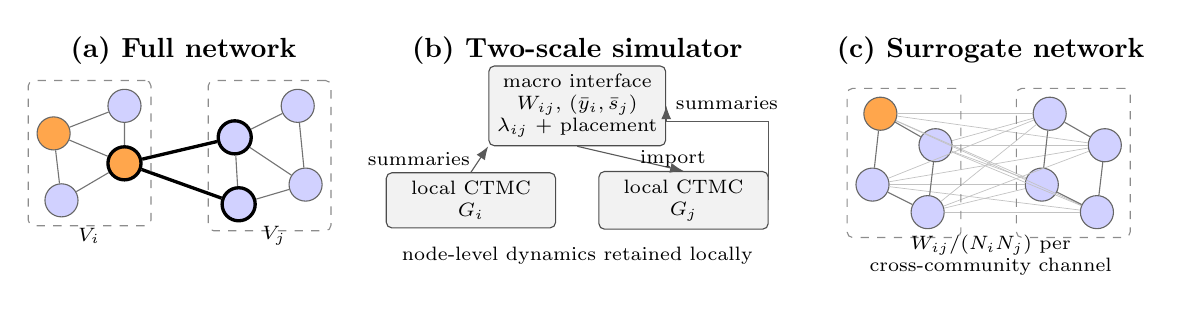
\begin{tikzpicture}[
  x=1cm,y=1cm,
  font=\scriptsize,
  >=Latex,
  person/.style={circle,draw=black!60,fill=blue!18,minimum size=4.2mm,inner sep=0pt},
  infected/.style={person,fill=orange!70},
  bridge/.style={person,very thick,draw=black},
  bridgeinf/.style={infected,very thick,draw=black},
  commbox/.style={draw=black!45,dashed,rounded corners=2pt,inner sep=3pt},
  macrobox/.style={draw=black!70,rounded corners=2pt,fill=black!5,align=center,inner sep=3pt},
  link/.style={draw=black!55},
  weak/.style={draw=black!24,line width=.25pt},
  flow/.style={-{Latex[length=1.7mm]},draw=black!65}
]
\node[font=\bfseries] at (0,2.25) {(a) Full network};
\node[infected] (a1) at (-1.65,1.20) {};
\node[person]   (a2) at (-1.55,0.35) {};
\node[bridgeinf](a3) at (-0.75,0.82) {};
\node[person]   (a4) at (-0.75,1.55) {};
\node[bridge]   (b1) at (0.65,1.15) {};
\node[person]   (b2) at (1.45,1.55) {};
\node[person]   (b3) at (1.55,0.55) {};
\node[bridge]   (b4) at (0.70,0.30) {};
\draw[link] (a1)--(a2)--(a3)--(a1) (a1)--(a4)--(a3);
\draw[link] (b1)--(b2)--(b3)--(b4)--(b1) (b1)--(b3);
\draw[very thick] (a3)--(b1);
\draw[very thick] (a3)--(b4);
\node[commbox,fit=(a1)(a2)(a3)(a4)] {};
\node[commbox,fit=(b1)(b2)(b3)(b4)] {};
\node at (-1.2,-0.10) {$V_i$};
\node at (1.15,-0.10) {$V_j$};

\node[font=\bfseries] at (5.0,2.25) {(b) Two-scale simulator};
\node[macrobox] (macro) at (5.0,1.55) {macro interface\\$W_{ij}$, $(\ibar_i,\sbar_j)$\\$\lambda_{ij}$ + placement};
\node[macrobox,minimum width=2.15cm,minimum height=.70cm] (li) at (3.65,0.35) {local CTMC\\$G_i$};
\node[macrobox,minimum width=2.15cm,minimum height=.70cm] (lj) at (6.35,0.35) {local CTMC\\$G_j$};
\draw[flow] (li.north) -- node[left] {summaries} (macro.south west);
\draw[flow] (macro.south) -- node[right] {import} (lj.north);
\draw[flow] (lj.east) -- ++(0,1.0) -| node[pos=1.08,right] {summaries} (macro.east);
\node at (5.0,-0.35) {node-level dynamics retained locally};

\node[font=\bfseries] at (10.25,2.25) {(c) Surrogate network};
\node[infected] (c1) at (8.85,1.45) {};
\node[person]   (c2) at (8.75,0.55) {};
\node[person]   (c3) at (9.55,1.05) {};
\node[person]   (c4) at (9.45,0.20) {};
\node[person]   (d1) at (11.00,1.45) {};
\node[person]   (d2) at (10.90,0.55) {};
\node[person]   (d3) at (11.70,1.05) {};
\node[person]   (d4) at (11.60,0.20) {};
\foreach \u in {c1,c2,c3,c4}{\foreach \v in {d1,d2,d3,d4}{\draw[weak] (\u)--(\v);}}
\draw[link] (c1)--(c2)--(c4)--(c3)--(c1);
\draw[link] (d1)--(d2)--(d4)--(d3)--(d1);
\node[commbox,fit=(c1)(c2)(c3)(c4)] {};
\node[commbox,fit=(d1)(d2)(d3)(d4)] {};
\node[align=center] at (10.25,-0.35) {$W_{ij}/(N_iN_j)$ per\\cross-community channel};
\end{tikzpicture}
\par\small\textbf{Рисунок 1. \textcolor{black}{Три подання зв'язку між спільнотами. (a) У повній мережі інфекція переходить лише через показані фізичні ребра та їхні вузли-мости. (b) Двомасштабний метод зберігає окремий локальний симулятор для кожної спільноти. Макрорівень отримує кількості вузлів у різних станах, використовує $W_{ij}$ для генерування міжспільнотного зараження та вибирає його ціль рівномірно серед сприйнятливих вузлів. (c) Ідеальний двомасштабний процес еквівалентний процесу на сурогатній мережі, де кожна напрямлена пара вузлів між двома спільнотами має слабкий зв'язок. Загальна вага всіх цих зв'язків дорівнює $W_{ij}$. Помаранчеві вузли --- інфіковані, сині --- сприйнятливі.}}

\end{minipage}\par
\end{minipage} &
\begin{minipage}[t]{\linewidth}
\par\noindent\begin{minipage}{\linewidth}
\color{black}\centering
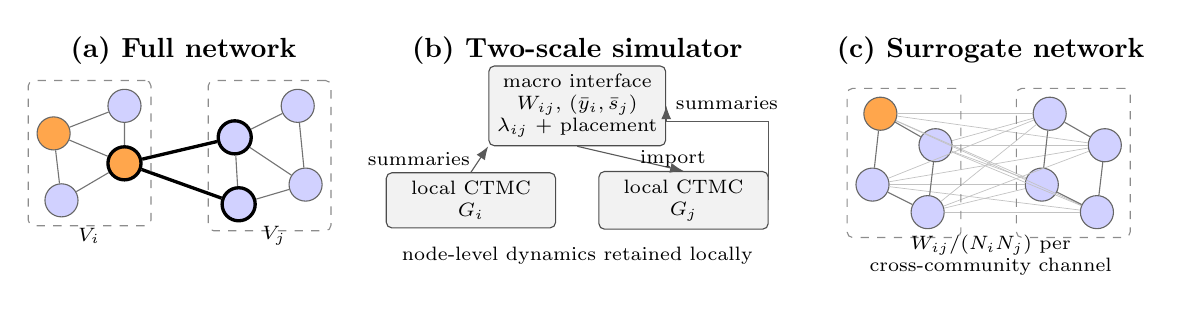
\begin{tikzpicture}[
  x=1cm,y=1cm,
  font=\scriptsize,
  >=Latex,
  person/.style={circle,draw=black!60,fill=blue!18,minimum size=4.2mm,inner sep=0pt},
  infected/.style={person,fill=orange!70},
  bridge/.style={person,very thick,draw=black},
  bridgeinf/.style={infected,very thick,draw=black},
  commbox/.style={draw=black!45,dashed,rounded corners=2pt,inner sep=3pt},
  macrobox/.style={draw=black!70,rounded corners=2pt,fill=black!5,align=center,inner sep=3pt},
  link/.style={draw=black!55},
  weak/.style={draw=black!24,line width=.25pt},
  flow/.style={-{Latex[length=1.7mm]},draw=black!65}
]
\node[font=\bfseries] at (0,2.25) {(a) Full network};
\node[infected] (a1) at (-1.65,1.20) {};
\node[person]   (a2) at (-1.55,0.35) {};
\node[bridgeinf](a3) at (-0.75,0.82) {};
\node[person]   (a4) at (-0.75,1.55) {};
\node[bridge]   (b1) at (0.65,1.15) {};
\node[person]   (b2) at (1.45,1.55) {};
\node[person]   (b3) at (1.55,0.55) {};
\node[bridge]   (b4) at (0.70,0.30) {};
\draw[link] (a1)--(a2)--(a3)--(a1) (a1)--(a4)--(a3);
\draw[link] (b1)--(b2)--(b3)--(b4)--(b1) (b1)--(b3);
\draw[very thick] (a3)--(b1);
\draw[very thick] (a3)--(b4);
\node[commbox,fit=(a1)(a2)(a3)(a4)] {};
\node[commbox,fit=(b1)(b2)(b3)(b4)] {};
\node at (-1.2,-0.10) {$V_i$};
\node at (1.15,-0.10) {$V_j$};

\node[font=\bfseries] at (5.0,2.25) {(b) Two-scale simulator};
\node[macrobox] (macro) at (5.0,1.55) {macro interface\\$W_{ij}$, $(\ibar_i,\sbar_j)$\\$\lambda_{ij}$ + placement};
\node[macrobox,minimum width=2.15cm,minimum height=.70cm] (li) at (3.65,0.35) {local CTMC\\$G_i$};
\node[macrobox,minimum width=2.15cm,minimum height=.70cm] (lj) at (6.35,0.35) {local CTMC\\$G_j$};
\draw[flow] (li.north) -- node[left] {summaries} (macro.south west);
\draw[flow] (macro.south) -- node[right] {import} (lj.north);
\draw[flow] (lj.east) -- ++(0,1.0) -| node[pos=1.08,right] {summaries} (macro.east);
\node at (5.0,-0.35) {node-level dynamics retained locally};

\node[font=\bfseries] at (10.25,2.25) {(c) Surrogate network};
\node[infected] (c1) at (8.85,1.45) {};
\node[person]   (c2) at (8.75,0.55) {};
\node[person]   (c3) at (9.55,1.05) {};
\node[person]   (c4) at (9.45,0.20) {};
\node[person]   (d1) at (11.00,1.45) {};
\node[person]   (d2) at (10.90,0.55) {};
\node[person]   (d3) at (11.70,1.05) {};
\node[person]   (d4) at (11.60,0.20) {};
\foreach \u in {c1,c2,c3,c4}{\foreach \v in {d1,d2,d3,d4}{\draw[weak] (\u)--(\v);}}
\draw[link] (c1)--(c2)--(c4)--(c3)--(c1);
\draw[link] (d1)--(d2)--(d4)--(d3)--(d1);
\node[commbox,fit=(c1)(c2)(c3)(c4)] {};
\node[commbox,fit=(d1)(d2)(d3)(d4)] {};
\node[align=center] at (10.25,-0.35) {$W_{ij}/(N_iN_j)$ per\\cross-community channel};
\end{tikzpicture}
\par\small\textbf{Рисунок 1. \textcolor{black}{Три подання зв'язку між спільнотами. (a) У повній мережі інфекція переходить лише через показані фізичні ребра та їхні вузли-мости. (b) Двомасштабний метод зберігає окремий локальний симулятор для кожної спільноти. Макрорівень отримує кількості вузлів у різних станах, використовує $W_{ij}$ для генерування міжспільнотного зараження та вибирає його ціль рівномірно серед сприйнятливих вузлів. (c) Ідеальний двомасштабний процес еквівалентний процесу на сурогатній мережі, де кожна напрямлена пара вузлів між двома спільнотами має слабкий зв'язок. Загальна вага всіх цих зв'язків дорівнює $W_{ij}$. Помаранчеві вузли --- інфіковані, сині --- сприйнятливі.}}

\end{minipage}\par
\end{minipage} \\[5mm]
\begin{minipage}[t]{\linewidth}
\subsection*{3.3. Локальні симулятори}

\end{minipage} &
\begin{minipage}[t]{\linewidth}
\subsection*{3.3. Локальні симулятори}

\end{minipage} \\*[5mm]
\begin{minipage}[t]{\linewidth}
Кожна спільнота має окремий симулятор Gillespie для свого графа $G_i$. Він застосовує інтенсивності зараження та видалення з~(2), використовуючи лише локальні ребра $E_{ii}$. Реалізація оновлює лише ті інтенсивності, на які вплинула остання подія, як у \citet{kuryliak2025simulating}. Кожен локальний симулятор має власний потік випадкових чисел.
\end{minipage} &
\begin{minipage}[t]{\linewidth}
Кожна спільнота має свій симулятор Gillespie для графа $G_i$. Він моделює зараження та видалення за~(2), враховуючи лише внутрішні контакти $E_{ii}$. Після події оновлюються лише ті інтенсивності, які вона змінила, як у \citet{kuryliak2025simulating}. Кожен симулятор має власний потік випадкових чисел.
\end{minipage} \\[5mm]
\begin{minipage}[t]{\linewidth}
Макрорівень може просунути локальний симулятор до заданого часу. Симулятор виконує локальні події до цього моменту. Потім макрорівень може імпортувати інфекцію, змінивши стан вибраного сприйнятливого вузла на $I$. Це змінює локальні інтенсивності. Реалізація зберігає невикористану частину випадкового порога наступної локальної події та перераховує час очікування за новою сумарною інтенсивністю. Тип події та її вузол вибираються за оновленими інтенсивностями. Новий локальний поріг генерується лише тоді, коли збереженого порога немає. Кожен локальний годинник має власний поріг, окремий від макропорога, описаного в Розділі~3.5. За заданих часів імпорту та цільових вузлів локальний симулятор виконує правила CTMC своєї мережі. Наближення виникає через спосіб генерування імпортів і вибору їхніх цільових вузлів.
\end{minipage} &
\begin{minipage}[t]{\linewidth}
Планувальник задає час, до якого локальний симулятор має виконати свої події. У цей момент він може додати імпорт: заразити вибраний сприйнятливий вузол. Після цього локальні інтенсивності змінюються. Симулятор зберігає невикористану частину випадкового порога наступної локальної події й перераховує час очікування за новою сумарною інтенсивністю. Подію та її вузол вибирає за оновленими інтенсивностями. Новий поріг генерує лише тоді, коли збереженого немає. Локальні пороги й поріг міжспільнотної події окремі; останній описано в Розділі~3.5. За заданих часів і цілей імпорту локальний симулятор точно виконує правила своєї мережі. Похибка зв'язування спільнот залежить від того, як планувальник визначає імпорти та вибирає їхні цілі.
\end{minipage} \\[5mm]
\begin{minipage}[t]{\linewidth}
\subsection*{3.4. Макрорівень}

\end{minipage} &
\begin{minipage}[t]{\linewidth}
\subsection*{3.4. Макрорівень}

\end{minipage} \\*[5mm]
\begin{minipage}[t]{\linewidth}
Макрорівень представляє спільноту її поточними частками вузлів, а напрямлений зв'язок --- вагою $W_{ij}$. Інтенсивність зараження зі спільноти $i$ до спільноти $j$:
\begin{equation*}\lambda_{ij}(t)=\beta_{\mathrm{out}}W_{ij}\ibar_i(t)\sbar_j(t),
\qquad \Theta(t)=\sum_{i\neq j}\lambda_{ij}(t).\tag{4}
\end{equation*}
Кожен множник має простий зміст. $\beta_{\mathrm{out}}W_{ij}$ задає загальну силу зв'язку; $\ibar_i$ --- частку інфікованих у спільноті-джерелі; $\sbar_j$ --- частку сприйнятливих у спільноті-одержувачі. Сума $\Theta$ --- інтенсивність будь-якого міжспільнотного зараження.
\end{minipage} &
\begin{minipage}[t]{\linewidth}
Планувальник використовує частки вузлів у різних станах і вагу $W_{ij}$. Інтенсивність передавання зі спільноти $i$ до спільноти $j$ дорівнює
\begin{equation*}\lambda_{ij}(t)=\beta_{\mathrm{out}}W_{ij}\ibar_i(t)\sbar_j(t),
\qquad \Theta(t)=\sum_{i\neq j}\lambda_{ij}(t).\tag{4}
\end{equation*}
Тут $\beta_{\mathrm{out}}W_{ij}$ задає загальну силу зв'язку, $\ibar_i$ --- частку інфікованих у джерелі, а $\sbar_j$ --- частку сприйнятливих в одержувачі. Що більше цих вузлів, то вища інтенсивність передавання. Сума $\Theta$ враховує всі напрямки між спільнотами.
\end{minipage} \\[5mm]
\begin{minipage}[t]{\linewidth}
Коли така подія відбувається, спочатку вибирають спільноту-джерело та спільноту-одержувача $(i,j)$ з імовірністю $\lambda_{ij}/\Theta$. Потім у спільноті $j$ рівномірно вибирають один сприйнятливий вузол і заражають його. Якщо таких вузлів 20, кожен має імовірність $1/20$. Вибір не враховує справжні вузли-мости, оскільки агрегований інтерфейс їх не знає. У подальших формулах цю імовірність позначаємо $\Pi_{ij}(v\mid x)=1/s_j$ для $v\in S_j$, де $x$ --- поточний стан мережі. Отже, $\Pi$ просто позначає імовірність вибору конкретного сприйнятливого вузла. Інші правила можливі, якщо є інформація про вузли-мости. Додатковий калібрувальний множник у реалізації дорівнює одиниці в усіх експериментах.
\end{minipage} &
\begin{minipage}[t]{\linewidth}
Коли така подія відбувається, спочатку вибирають спільноту-джерело та спільноту-одержувача $(i,j)$ з імовірністю $\lambda_{ij}/\Theta$. Потім у спільноті $j$ рівномірно вибирають один сприйнятливий вузол і заражають його. Якщо таких вузлів 20, кожен має імовірність $1/20$. Вибір не враховує справжні вузли-мости, оскільки агрегований інтерфейс їх не знає. У подальших формулах цю імовірність позначаємо $\Pi_{ij}(v\mid x)=1/s_j$ для $v\in S_j$, де $x$ --- поточний стан мережі. Отже, $\Pi$ просто позначає імовірність вибору конкретного сприйнятливого вузла. Інші правила можливі, якщо є інформація про вузли-мости. Додатковий калібрувальний множник у реалізації дорівнює одиниці в усіх експериментах.
\end{minipage} \\[5mm]
\begin{minipage}[t]{\linewidth}
Ця агрегована інтенсивність загалом наближено описує передавання через справжні фізичні ребра. Для заданих кількостей вузлів у станах вона дорівнює очікуваній інтенсивності за рівномірного випадкового вибору кінців ребер, перш ніж враховано їхні конкретні ідентичності, стани та історію епідемії. Це не гарантує правильної інтенсивності для вже реалізованої епідемії на конкретних ребрах. Для рівномірного зв'язку «усі з усіма» вона є фактичною інтенсивністю, як пояснено в Розділі~4. Значення $\Theta$ змінюється після локальної події або імпорту, які змінюють кількості вузлів у станах.
\end{minipage} &
\begin{minipage}[t]{\linewidth}
Формула усереднює передавання між спільнотами. За заданих кількостей інфікованих і сприйнятливих вона дорівнює очікуваній інтенсивності, якщо кінці міжспільнотних ребер вибрати рівномірно й випадково. Для конкретної мережі інтенсивність може бути іншою: важливі стани саме вузлів із міжспільнотними контактами та історія заражень. Для сурогатної мережі зі зв'язками «усі з усіма» формула точна (Розділ~4). Значення $\Theta$ оновлюється після подій, що змінюють кількості вузлів у різних станах.
\end{minipage} \\[5mm]
\begin{minipage}[t]{\linewidth}
\subsection*{3.5. Час подій та синхронізація}

\end{minipage} &
\begin{minipage}[t]{\linewidth}
\subsection*{3.5. Час подій та синхронізація}

\end{minipage} \\*[5mm]
\begin{minipage}[t]{\linewidth}
Після макроподії в час $t_0$ генеруємо випадковий поріг $E\sim\Exp(1)$: експоненційне випадкове число із середнім один. Починаючи з нуля, накопичуємо загальну інтенсивність $\Theta$. Наступна макроподія відбувається в перший момент $t^\ast$, коли накопичена величина досягає $E$:
\begin{equation*}\int_{t_0}^{t^\ast}\Theta(s)\,ds=E.\tag{5}
\end{equation*}
Інакше кажучи, площа під кривою інтенсивності зростає до випадкового порога. Якщо поріг не досягнуто, наступної макроподії немає. Це стандартний спосіб визначення часу події за накопиченою інтенсивністю \citep{ethier1986,anderson2007}. За сталої $\Theta$ час очікування дорівнює $E/\Theta$. Якщо згенерувати $E=-\ln U$, де $U$ рівномірно розподілене на $(0,1)$, отримуємо звичний час очікування Gillespie. Коли локальна подія змінює $\Theta$, зберігаємо той самий поріг і продовжуємо накопичення з новою інтенсивністю. Новий макропоріг генеруємо лише після макроподії. Це той самий годинник за накопиченою інтенсивністю, який описано в конференційній роботі. Точне визначення першого досягнення порога задає ідеальний процес; описаний нижче розрахунок на часовій сітці наближено визначає цей момент. У Розділі~4.1 показано, що ідеальний процес точний для сурогатної мережі.
\end{minipage} &
\begin{minipage}[t]{\linewidth}
Після міжспільнотного зараження в час $t_0$ генеруємо випадковий поріг $E\sim\Exp(1)$ --- експоненційне число із середнім один. Від цього моменту накопичуємо загальну інтенсивність $\Theta$. Наступне міжспільнотне зараження відбувається в перший момент $t^\ast$, коли накопичена величина досягає порога:
\begin{equation*}\int_{t_0}^{t^\ast}\Theta(s)\,ds=E.\tag{5}
\end{equation*}
Інтеграл --- це площа під кривою інтенсивності. Вона зростає до порога $E$; якщо його не досягнуто, подія не відбувається. Так визначають час події за змінної інтенсивності \citep{ethier1986,anderson2007}. За сталої $\Theta$ час очікування дорівнює $E/\Theta$. Якщо взяти $E=-\ln U$, де $U$ рівномірно розподілене на $(0,1)$, отримуємо звичну формулу Gillespie. Коли локальна подія змінює $\Theta$, зберігаємо поріг і вже накопичену величину, а далі додаємо внесок нової інтенсивності. Новий поріг генеруємо після міжспільнотного зараження. Цей принцип використано і в конференційній роботі. Ідеальний процес визначає момент досягнення порога точно; наша реалізація оцінює його за часовою сіткою. Ідеальний процес точний для сурогатної мережі (Розділ~4.1).
\end{minipage} \\[5mm]
\begin{minipage}[t]{\linewidth}
Реалізований планувальник узгоджує локальні симулятори на інтервалах довжини $\tau$. У конференційному описі цього годинника також використано оцінку інтенсивності в середині кроку. Тут уточнюємо, як отримати її від локальних симуляторів. Нехай $A$ --- уже накопичена величина від попередньої макроподії. Для поточного інтервалу $[t,t_g)$ копіюємо кожен локальний симулятор разом зі станом генератора випадкових чисел і просуваємо копію до середини інтервалу. За копіями обчислюємо оцінку загальної макроінтенсивності $\Theta_{\mathrm{mid}}$. Оцінений приріст за залишок інтервалу дорівнює $\Theta_{\mathrm{mid}}(t_g-t)$. Якщо $A$ плюс цей приріст менше за $E$ (випадковий макропоріг), справжні симулятори просуваються до $t_g$. Інакше час події оцінюємо як
\begin{equation*}t^\ast=t+\frac{E-A}{\Theta_{\mathrm{mid}}}.\tag{6}
\end{equation*}
Тут $E$ --- випадковий макропоріг, а $A$ --- уже накопичена до нього величина. Чисельник $E-A$ --- залишок до порога; ділення на оцінену інтенсивність дає залишковий час очікування. Наприклад, за $E=1$, $A=0.4$ та $\Theta_{\mathrm{mid}}=0.2$ оцінений час очікування дорівнює трьом одиницям часу. Планувальник просуває справжні симулятори до $t^\ast$, за їхніми станами в цей момент вибирає спільноту-джерело та спільноту-одержувача, вибирає сприйнятливий цільовий вузол і застосовує зараження. Повну послідовність наведено в Алгоритмі~1.
\end{minipage} &
\begin{minipage}[t]{\linewidth}
У реалізації час поділено на інтервали довжини $\tau$. Час міжспільнотного зараження може лежати всередині інтервалу: його не округлюють до точки сітки. Для оцінки використовуємо інтенсивність у середині інтервалу, як у конференційному описі. Позначимо через $A$ уже накопичену величину. На поточному інтервалі $[t,t_g)$ копіюємо локальні симулятори разом зі станами їхніх генераторів випадкових чисел. Копії виконуємо до середини інтервалу й за їхніми станами обчислюємо $\Theta_{\mathrm{mid}}$. Оцінка приросту дорівнює $\Theta_{\mathrm{mid}}(t_g-t)$. Якщо $A$ разом із цим приростом ще менше за $E$, справжні симулятори виконуються до $t_g$. Інакше оцінюємо час зараження:
\begin{equation*}t^\ast=t+\frac{E-A}{\Theta_{\mathrm{mid}}}.\tag{6}
\end{equation*}
Залишок до порога дорівнює $E-A$. Ділення на оцінену інтенсивність дає час, потрібний для його накопичення. Наприклад, якщо $E=1$, $A=0.4$ і $\Theta_{\mathrm{mid}}=0.2$, час очікування дорівнює трьом одиницям часу. Планувальник виконує справжні симулятори до $t^\ast$ і за їхніми станами вибирає напрямок передавання та сприйнятливий вузол-одержувач. Потім заражає цей вузол. Повну послідовність наведено в Алгоритмі~1.
\end{minipage} \\[5mm]
\begin{minipage}[t]{\linewidth}
\par\noindent\begin{minipage}{\linewidth}
\color{black}
\par\small\textbf{Алгоритм 1. \textcolor{black}{Один запуск двомасштабного симулятора з узгодженням за часовою сіткою.}}

\small
\fbox{\begin{minipage}{0.94\linewidth}
\textbf{Вхід:} локальні графи $G_i$, ваги $W_{ij}$, інтенсивності, крок $\tau$, горизонт $T_{\mathrm{end}}$ та початковий стан.
\begin{enumerate}
\item Установити $t=0$ і $A=0$; згенерувати $E\sim\Exp(1)$.
\item Поки $t<T_{\mathrm{end}}$ й інфекція може поширюватися, встановити $t_g=\min(t+\tau,T_{\mathrm{end}})$ та обробити інтервал до $t_g$.
\item Скопіювати кожен локальний симулятор разом зі станом генератора випадкових чисел. Просунути копії до середини залишку інтервалу та обчислити $\Theta_{\mathrm{mid}}$ за~(4).
\item Якщо $A+\Theta_{\mathrm{mid}}(t_g-t)<E$, просунути справжні симулятори до $t_g$, додати цю величину до $A$, встановити $t=t_g$ і повернутися до кроку 2.
\item Інакше обчислити $t^\ast$ за~(6) та просунути справжні симулятори до $t^\ast$.
\item Вибрати $(i,j)$ з імовірністю $\lambda_{ij}(t^\ast)/\Theta(t^\ast)$. Рівномірно вибрати $v$ з $S_j(t^\ast)$ та імпортувати зараження у $v$. Оновити локальний симулятор одержувача, зберігаючи невикористаний експоненційний поріг і вибираючи локальну подію за новими інтенсивностями.
\item Установити $t=t^\ast$ і $A=0$, згенерувати нове $E\sim\Exp(1)$ та так само обробити залишок поточного інтервалу.
\end{enumerate}
\end{minipage}}
\end{minipage}\par
\end{minipage} &
\begin{minipage}[t]{\linewidth}
\par\noindent\begin{minipage}{\linewidth}
\color{black}
\par\small\textbf{Алгоритм 1. \textcolor{black}{Один запуск двомасштабного симулятора з узгодженням за часовою сіткою.}}

\small
\fbox{\begin{minipage}{0.94\linewidth}
\textbf{Вхід:} локальні графи $G_i$, ваги $W_{ij}$, інтенсивності, крок $\tau$, горизонт $T_{\mathrm{end}}$ та початковий стан.
\begin{enumerate}
\item Установити $t=0$ і $A=0$; згенерувати $E\sim\Exp(1)$.
\item Поки $t<T_{\mathrm{end}}$ й інфекція може поширюватися, встановити $t_g=\min(t+\tau,T_{\mathrm{end}})$ та обробити інтервал до $t_g$.
\item Скопіювати кожен локальний симулятор разом зі станом генератора випадкових чисел. Просунути копії до середини залишку інтервалу та обчислити $\Theta_{\mathrm{mid}}$ за~(4).
\item Якщо $A+\Theta_{\mathrm{mid}}(t_g-t)<E$, просунути справжні симулятори до $t_g$, додати цю величину до $A$, встановити $t=t_g$ і повернутися до кроку 2.
\item Інакше обчислити $t^\ast$ за~(6) та просунути справжні симулятори до $t^\ast$.
\item Вибрати $(i,j)$ з імовірністю $\lambda_{ij}(t^\ast)/\Theta(t^\ast)$. Рівномірно вибрати $v$ з $S_j(t^\ast)$ та імпортувати зараження у $v$. Оновити локальний симулятор одержувача, зберігаючи невикористаний експоненційний поріг і вибираючи локальну подію за новими інтенсивностями.
\item Установити $t=t^\ast$ і $A=0$, згенерувати нове $E\sim\Exp(1)$ та так само обробити залишок поточного інтервалу.
\end{enumerate}
\end{minipage}}
\end{minipage}\par
\end{minipage} \\[5mm]
\begin{minipage}[t]{\linewidth}
Копіювання станів генераторів випадкових чисел важливе: якщо до середини інтервалу не відбудеться імпорт, копія відтворить ту саму траєкторію, що й справжній симулятор. Оцінка середньої точки точна на інтервалі без локальних подій. Її похибка визначення часу та використання майбутнього стану не більш як на $\tau/2$ зникають зі зменшенням $\tau$ до нуля.
\end{minipage} &
\begin{minipage}[t]{\linewidth}
Копії використовують той самий стан генератора випадкових чисел, що й справжні симулятори. Тому до першого імпорту вони відтворюють ту саму локальну траєкторію. Якщо на інтервалі немає локальних подій, інтенсивність стала й оцінка за серединою інтервалу точна. Якщо такі події є, оцінка може використати стан, пізніший за оцінений час імпорту, не більш ніж на $\tau/2$. Менший крок зменшує цей часовий зсув; у границі $\tau\to0$ похибка сітки зникає.
\end{minipage} \\[5mm]
\begin{minipage}[t]{\linewidth}
Часова сітка потрібна, оскільки планувальник працює з локальними симуляторами як із «чорними скриньками». Якщо вони також повідомляють часи наступних локальних подій, планувальник може об'єднати ці часи та точно накопичувати $\Theta$, яка стала між подіями. Такий подієвий варіант усуває чисельну похибку синхронізації. В експериментах цієї статті використано реалізований сітковий варіант із $\tau=1$.
\end{minipage} &
\begin{minipage}[t]{\linewidth}
Щоб обійтися без часової сітки, локальні симулятори мають повідомляти часи своїх наступних подій. Тоді планувальник може обробляти події в часовому порядку й точно накопичувати $\Theta$, яка стала між подіями. Імпорт застосовується в момент його виникнення, після чого локальні інтенсивності оновлюються. Такий варіант усуває похибку часової синхронізації, але зберігає усереднений опис міжспільнотних зв'язків. В експериментах використано варіант із часовою сіткою та кроком $\tau=1$.
\end{minipage} \\[5mm]
\begin{minipage}[t]{\linewidth}
\subsection*{3.6. Обчислювальна структура та застосування}

\end{minipage} &
\begin{minipage}[t]{\linewidth}
\subsection*{3.6. Обчислювальна структура та застосування}

\end{minipage} \\*[5mm]
\begin{minipage}[t]{\linewidth}
\Full{} зберігає всі локальні та міжспільнотні канали, а обсяг роботи на одну подію зростає зі степенем вузла \citep{kuryliak2025simulating}. \TS{} зберігає локальні графи та матрицю загальних ваг розміру $M\times M$. У конференційній роботі обговорено таке скорочення даних про міжспільнотні контакти \citep{kuryliak2025towards}. Його значення залежить від задачі. Заміна багатьох індивідуальних міжспільнотних ребер однією вагою може зменшити обсяг збережених даних. Якщо таких ребер лише кілька, економія може бути малою; локальні графи все одно потрібно зберігати.
\end{minipage} &
\begin{minipage}[t]{\linewidth}
\Full{} зберігає всі контакти, зокрема між спільнотами. Обсяг роботи після події залежить від кількості сусідів відповідного вузла \citep{kuryliak2025simulating}. \TS{} зберігає локальні графи та матрицю міжспільнотних ваг розміру $M\times M$. Таке скорочення даних обговорено в конференційній роботі \citep{kuryliak2025towards}. Якщо міжспільнотних ребер багато, заміна їх загальними вагами може зменшити обсяг даних. Якщо ребер мало, економія може бути незначною. Локальні графи в будь-якому разі потрібно зберігати.
\end{minipage} \\[5mm]
\begin{minipage}[t]{\linewidth}
Окремі локальні симулятори також створюють можливість паралельного виконання. Коли планувальник визначив наступний цільовий час ($t_g$ або $t^\ast$), локальні симулятори можна незалежно просунути до цього самого часу. Копії для оцінки середньої точки також можна обробляти паралельно. Потім макрорівень має зібрати кількості вузлів і застосувати імпорт, якщо він запланований, перш ніж продовжувати. У досліджуваній реалізації локальні симулятори просуваються послідовно; паралельне виконання в межах одного запуску є можливим розширенням, а не виміряним прискоренням. Локальні симулятори також можуть мати різні налаштування для різних спільнот.
\end{minipage} &
\begin{minipage}[t]{\linewidth}
Локальні симулятори можна виконувати паралельно до спільного часу $t_g$ або $t^\ast$, який уже визначив планувальник. Копії для оцінки інтенсивності також можна виконувати паралельно. Потім потрібно зібрати стани спільнот і застосувати імпорт, якщо він має відбутися. У нашій реалізації локальні симулятори виконуються послідовно; можливе паралельне виконання ще не дає підстав заявляти про прискорення. Для різних спільнот також можна задавати різні локальні налаштування.
\end{minipage} \\[5mm]
\begin{minipage}[t]{\linewidth}
Сітковий планувальник додає роботу через копіювання локальних станів та узгодження спільнот. Тому ні менше використання пам'яті, ні швидше виконання не гарантовані. Метод корисний, коли конкретні міжспільнотні контакти недоступні або надто численні для явного подання. Виміряний час виконання наведено в Розділі~7.2; головний предмет цієї статті --- похибка наближення.
\end{minipage} &
\begin{minipage}[t]{\linewidth}
Копіювання станів і синхронізація потребують додаткової роботи, тому метод не гарантує меншого використання пам'яті або швидшого виконання. Його можна застосовувати, коли конкретні міжспільнотні контакти невідомі або їх надто багато для явного зберігання. Час виконання наведено в Розділі~7.2. Основне питання цієї статті --- точність такого спрощення.
\end{minipage} \\[5mm]
\begin{minipage}[t]{\linewidth}
\section*{4. Що агрегований інтерфейс зберігає, а що втрачає}

\end{minipage} &
\begin{minipage}[t]{\linewidth}
\section*{4. Що насправді моделює двомасштабний метод}

\end{minipage} \\*[5mm]
\begin{minipage}[t]{\linewidth}
\subsection*{4.1. Представлення за допомогою сурогатної мережі}

\end{minipage} &
\begin{minipage}[t]{\linewidth}
\subsection*{4.1. Точність для усередненої мережі}

\end{minipage} \\*[5mm]
\begin{minipage}[t]{\linewidth}
За точного обчислення часу~(5) ідеальний двомасштабний процес є CTMC на $\{S,I,R\}^V$. Інтенсивність його переходу $x\to x^{v:I}$ унаслідок імпорту дорівнює $\sum_{i\neq j}\lambda_{ij}(x)\Pi_{ij}(v\mid x)$ для $v\in S_j(x)$; усі локальні переходи мають інтенсивності з~(2), обмежені на $E_{ii}$. Наступне твердження ототожнює цей процес із процесом на повній мережі зі зміненим графом.
\end{minipage} &
\begin{minipage}[t]{\linewidth}
Якщо визначати час кожної події точно за~(5), двомасштабний метод сам задає неперервний марковський ланцюг. Він має ті самі локальні правила зараження й видалення, що й повний Gillespie. Відмінність стосується контактів між спільнотами. Замість справжніх ребер метод фактично використовує слабкі зв'язки між усіма парами вузлів двох зв'язаних спільнот. Таку усереднену мережу називаємо сурогатною й позначаємо $\tilde G$.
\par Для сприйнятливого вузла $v\in V_j$ інтенсивність імпорту дорівнює $\sum_{i\neq j}\lambda_{ij}(x)\Pi_{ij}(v\mid x)$. Наступне твердження показує, що це саме інтенсивність зараження вузла в $\tilde G$.
\end{minipage} \\[5mm]
\begin{minipage}[t]{\linewidth}
\par\noindent\textbf{Твердження 1 (Сурогатна мережа).}\par\noindent 
Нехай $\tilde G$ --- мережа з тими самими внутрішньоспільнотними каналами та інтенсивностями, що й $G$, у якій кожен міжспільнотний пучок $E_{ij}$ замінено повною множиною каналів $V_i\times V_j$, кожен з інтенсивністю $\tilde\beta_{uv}=\beta_{\mathrm{out}}W_{ij}/(N_iN_j)$. За рівномірного розміщення ідеальний двомасштабний процес має генератор $\mathcal{L}_{\tilde G}$; тобто він має закон процесу на повній мережі $\tilde G$, запущеного з тієї самої конфігурації.
\par
\end{minipage} &
\begin{minipage}[t]{\linewidth}
\par\noindent\textbf{Твердження 1 (Точна модель для сурогатної мережі).}\par\noindent 
Нехай $\tilde G$ має ті самі внутрішні контакти та інтенсивності, що й $G$. Для кожної пари спільнот $i\neq j$ замінимо її справжні міжспільнотні канали $E_{ij}$ усіма каналами $V_i\times V_j$. Кожному новому каналу надамо інтенсивність $\tilde\beta_{uv}=\beta_{\mathrm{out}}W_{ij}/(N_iN_j)$. Якщо симулятор вибирає ціль імпорту рівномірно серед сприйнятливих вузлів, ідеальний двомасштабний процес має генератор $\mathcal{L}_{\tilde G}$. Отже, за однакового початкового стану його розподіл збігається з розподілом повного Gillespie на $\tilde G$.
\par
\end{minipage} \\[5mm]
\begin{minipage}[t]{\linewidth}
\par\noindent\textit{Доведення.}\par\noindent 
Видалення та внутрішньоспільнотні зараження мають однакові інтенсивності в обох процесах. Розглянемо сприйнятливий вузол $v\in V_j$ у конфігурації $x$. За рівномірного розміщення двомасштабна інтенсивність, з якою $v$ заражається внаслідок імпорту, дорівнює
\[\fitmath{\sum_{i\neq j}\lambda_{ij}(x)\,\frac{1}{s_j(x)}
=\sum_{i\neq j}\beta_{\mathrm{out}}W_{ij}\frac{y_i(x)}{N_i}\frac{s_j(x)}{N_j}\frac{1}{s_j(x)}
=\sum_{i\neq j}\sum_{u\in V_i}\frac{\beta_{\mathrm{out}}W_{ij}}{N_iN_j}\ind\{x_u=I\},}\]
що є сумарною інтенсивністю міжспільнотних каналів $\tilde G$, спрямованих у $v$. Коли $s_j(x)=0$, обидві інтенсивності дорівнюють нулю. Отже, всі інтенсивності переходів збігаються, а генератори є однаковими. \qed
\par
\end{minipage} &
\begin{minipage}[t]{\linewidth}
\par\noindent\textit{Доведення.}\par\noindent 
Локальні зараження та видалення мають однакові інтенсивності. Для сприйнятливого вузла $v\in V_j$ імовірність вибору ціллю імпорту дорівнює $1/s_j(x)$. Тому його інтенсивність зараження з інших спільнот дорівнює
\[\fitmath{\begin{aligned}
\sum_{i\neq j}\lambda_{ij}(x)\frac{1}{s_j(x)}
&=\sum_{i\neq j}\beta_{\mathrm{out}}W_{ij}\frac{y_i(x)}{N_i}\frac{s_j(x)}{N_j}\frac{1}{s_j(x)}\\
&=\sum_{i\neq j}\sum_{u\in V_i}\frac{\beta_{\mathrm{out}}W_{ij}}{N_iN_j}\ind\{x_u=I\}.
\end{aligned}}\]
Останній вираз підсумовує інтенсивності всіх каналів $\tilde G$, що ведуть від інфікованих вузлів до $v$. Якщо $s_j(x)=0$, імпорт неможливий в обох моделях. Отже, всі інтенсивності переходів збігаються. \qed
\par
\end{minipage} \\[5mm]
\begin{minipage}[t]{\linewidth}
\par\noindent\textbf{Наслідок 1.}\par\noindent 
Якщо кожен міжспільнотний пучок у $G$ уже є повним, $E_{ij}=V_i\times V_j$, зі спільною інтенсивністю для кожної пари спільнот, тоді $\tilde G=G$, а ідеальний двомасштабний процес є точним.
\par
\end{minipage} &
\begin{minipage}[t]{\linewidth}
\par\noindent\textbf{Наслідок 1.}\par\noindent 
Якщо в початковій мережі кожен вузол спільноти $i$ вже з'єднаний із кожним вузлом спільноти $j$, а всі ці канали мають однакову інтенсивність для даної пари спільнот, то $\tilde G=G$. У цьому випадку ідеальний двомасштабний метод точний і для початкової мережі.
\par
\end{minipage} \\[5mm]
\begin{minipage}[t]{\linewidth}
Сурогатна мережа зберігає сумарну вагу кожного пучка, $\sum_{(u,v)\in V_i\times V_j}\tilde\beta_{uv}=\beta_{\mathrm{out}}W_{ij}$, але рівномірно розподіляє її між усіма парами (рисунок~1c). Тому похибка апроксимації ідеального методу є різницею між епідеміями на $G$ та $\tilde G$, які відрізняються лише своїми інтерфейсами. Реалізований метод додає чисельну похибку синхронізації. Твердження~1 також дає практичний спосіб верифікації: для малих мереж похибку синхронізації можна виокремити, порівнюючи двомасштабний симулятор із точною симуляцією на $\tilde G$.
\end{minipage} &
\begin{minipage}[t]{\linewidth}
Загальна сила зв'язку зберігається:
\[\fitmath{\sum_{(u,v)\in V_i\times V_j}\tilde\beta_{uv}=\beta_{\mathrm{out}}W_{ij}.}\]
Змінюється її розподіл між вузлами (Рисунок~1c). Тому навіть за точного часу подій результати на $G$ і $\tilde G$ можуть відрізнятися. Реалізація з часовою сіткою додає ще й чисельну похибку. Ці два ефекти можна перевіряти окремо: порівняння з повним Gillespie на $\tilde G$ перевіряє синхронізацію, а порівняння з повним Gillespie на $G$ показує також наслідки заміни контактів.
\end{minipage} \\[5mm]
\begin{minipage}[t]{\linewidth}
\subsection*{4.2. Джерела розбіжностей}

\end{minipage} &
\begin{minipage}[t]{\linewidth}
\subsection*{4.2. Звідки виникає похибка}

\end{minipage} \\*[5mm]
\begin{minipage}[t]{\linewidth}
Порівняння $G$ із $\tilde G$ виявляє чотири механізми, через які двомасштабний симулятор може відхилятися від процесу на повній мережі.
\end{minipage} &
\begin{minipage}[t]{\linewidth}
Заміна справжніх міжспільнотних контактів усередненими змінює три речі: інтенсивність передавання, вузол-одержувач і можливу кількість імпортів. Четверте джерело похибки --- наближене визначення часу подій у реалізації.
\end{minipage} \\[5mm]
\begin{minipage}[t]{\linewidth}
\paragraph{Інформація про стан межі (з боку джерела).}
У $G$ інтенсивність передавання з $V_i$ до $V_j$ дорівнює
\begin{equation*}a^\star_{ij}(x)=\beta_{\mathrm{out}}\sum_{(u,v)\in E_{ij}}w_{uv}\,\ind\{x_u=I,\,x_v=S\},\tag{7}
\end{equation*}
і залежить від того, чи заражені конкретні мостові вузли. У $\tilde G$ свій внесок робить кожен заражений вузол $V_i$. Тому експорти можуть відбуватися до зараження будь-якого мостового вузла. Такий \emph{обхід мостів} неможливий у $G$ і дає безпосередній діагностичний показник (розділ~4.3).
\end{minipage} &
\begin{minipage}[t]{\linewidth}
\paragraph{1. Не враховано стан справжніх вузлів-мостів.}
У повній мережі інтенсивність передавання з $V_i$ до $V_j$ дорівнює
\begin{equation*}a^\star_{ij}(x)=\beta_{\mathrm{out}}\sum_{(u,v)\in E_{ij}}w_{uv}\,\ind\{x_u=I,\,x_v=S\},\tag{7}
\end{equation*}
Тут у суму входять лише контакти від інфікованого вузла до сприйнятливого. Якщо всі вузли-мости в джерелі ще сприйнятливі, передавання неможливе. У двомасштабному методі інтенсивність залежить від загальної частки інфікованих, тому зараження будь-якого вузла джерела може сприяти експорту. Метод може передати інфекцію, поки жоден справжній міст ще не заражений. Далі називаємо це \emph{обходом мостів} (Розділ~4.3).
\end{minipage} \\[5mm]
\begin{minipage}[t]{\linewidth}
\paragraph{Розміщення (з боку приймача).}
У $G$ передавання заражає цільову кінцеву вершину каналу, що спрацював; у $\tilde G$ ціль рівномірно вибирається серед сприйнятливих вузлів. Місце імпорту визначає його відстань до наступного інтерфейсу, а отже, і час подальших переходів.
\end{minipage} &
\begin{minipage}[t]{\linewidth}
\paragraph{2. Змінено місце зараження в одержувачі.}
У повній мережі заражається вузол на кінці контакту, через який прийшла інфекція. Двомасштабний метод вибирає будь-який сприйнятливий вузол з однаковою імовірністю. Від цього залежить, як швидко інфекція дійде до вузлів-мостів, що ведуть у наступну спільноту.
\end{minipage} \\[5mm]
\begin{minipage}[t]{\linewidth}
\paragraph{Вичерпання інтерфейсу (з боку приймача).}
За SI-динаміки канал $G$ передає зараження не більш ніж один раз: після цього його ціль заражена. Тому пучок із $|E_{ij}|$ каналів переносить не більш ніж $|E_{ij}|$ заражень, а інтерфейс з одним ребром --- рівно одне. У $\tilde G$ імпорти з $V_i$ у $V_j$ тривають з інтенсивністю $\lambda_{ij}=\beta_{\mathrm{out}}W_{ij}\ibar_i\sbar_j$, доки $V_j$ не буде вичерпано; їхня очікувана кількість за період $[t_1,t_2]$ дорівнює $\mathbb{E}\int_{t_1}^{t_2}\lambda_{ij}(s)\,ds$. Отже, коли приймальна спільнота тривалий час залишається переважно сприйнятливою, двомасштабний симулятор продовжує засівати її додатковими зараженнями, яких повна мережа передати не може.
\end{minipage} &
\begin{minipage}[t]{\linewidth}
\paragraph{3. Можливі додаткові імпорти.}
У SI-моделі вузол після зараження залишається інфікованим. Тому один справжній напрямлений канал може заразити свій цільовий вузол не більше одного разу. Через $|E_{ij}|$ каналів можливі не більше $|E_{ij}|$ заражень; через один канал --- не більше одного.
\par У сурогатній мережі контактів значно більше. Інтенсивність $\lambda_{ij}=\beta_{\mathrm{out}}W_{ij}\ibar_i\sbar_j$ може залишатися додатною після першого імпорту. Очікувана кількість імпортів на інтервалі $[t_1,t_2]$ дорівнює $\mathbb{E}\int_{t_1}^{t_2}\lambda_{ij}(s)\,ds$. Якщо одержувач довго залишається переважно сприйнятливим, метод може додавати зараження, які неможливі через початковий набір контактів.
\end{minipage} \\[5mm]
\begin{minipage}[t]{\linewidth}
\paragraph{Синхронізація.}
Квадратурна формула середньої точки та інтерполяція з розділу~3.5 апроксимують~(5).
\end{minipage} &
\begin{minipage}[t]{\linewidth}
\paragraph{4. Час події обчислюється наближено.}
Реалізація оцінює інтенсивність за станом у середині інтервалу й використовує цю оцінку для визначення часу імпорту (Розділ~3.5). Так вона наближено обчислює інтеграл у~(5). Ця похибка стосується часової сітки й залишається окремою від заміни контактів.
\end{minipage} \\[5mm]
\begin{minipage}[t]{\linewidth}
\par\noindent\textbf{Зауваження 1 (Розміщення за рандомізованих інтерфейсів).}\par\noindent 
Припустімо, що кінцеві вершини кожного пучка вибираються рівномірно й незалежно від внутрішніх графів та кінцевих вершин інших пучків, як у наведених нижче експериментах. Тоді ціль першого передавання до повністю сприйнятливої спільноти має рівномірний розподіл і в $G$, оскільки вона є кінцевою вершиною рівномірно розміщеного каналу, і в $\tilde G$. Тому розміщення може впливати на часи прибуття лише через передавання після першого. У таких схемах відмінності між першим і подальшими переходами виокремлюють ефекти з боку приймача (розділ~6.6).
\par
\end{minipage} &
\begin{minipage}[t]{\linewidth}
\par\noindent\textbf{Зауваження 1 (Перший імпорт за випадкового розміщення контактів).}\par\noindent 
Нехай кінці міжспільнотних каналів вибрано рівномірно й незалежно від внутрішніх графів та інших наборів контактів, як у наших тестах. Якщо спільнота-одержувач ще повністю сприйнятлива, ціль її першого імпорту також рівномірна в повній мережі --- після усереднення за випадковим розміщенням контактів. Двомасштабний метод має такий самий розподіл першої цілі. Для окремої зафіксованої мережі цілі не мусять збігатися. Однаковий розподіл першої цілі також не означає однакового розподілу часу першого імпорту. Порівняння першого й наступних переходів допомагає дослідити наслідки подальшого вибору цілей і додаткових імпортів (Розділ~6.6).
\par
\end{minipage} \\[5mm]
\begin{minipage}[t]{\linewidth}
\subsection*{4.3. Одиничний експорт: стохастичне впорядкування та обхід мостів}

\end{minipage} &
\begin{minipage}[t]{\linewidth}
\subsection*{4.3. Одне передавання інфекції назовні}

\end{minipage} \\*[5mm]
\begin{minipage}[t]{\linewidth}
Розглянемо спільноту-джерело $V_0$ розміру $n$ із довільним внутрішнім графом, SI-динамікою та єдиним сприйнятливим листковим вузлом $\ell$, сполученим із множиною $B\subset V_0$ з $k$ мостових вузлів каналами з інтенсивністю $\beta_{\mathrm{out}}$. Тоді $W_{0\ell}=k$, а до експорту $\sbar_\ell=1$, тому $\lambda_{0\ell}=\beta_{\mathrm{out}}k\,\ibar_0$. Нехай $\tau_u$ --- час зараження вузла $u$, $A_u(t)=(t-\tau_u)^+$ --- тривалість його перебування в зараженому стані, а $T_B=\min_{u\in B}\tau_u$.
\end{minipage} &
\begin{minipage}[t]{\linewidth}
Щоб окремо розглянути передавання з джерела, приєднаємо до спільноти $V_0$ з $n$ вузлів один сприйнятливий вузол $\ell$. Такий зовнішній вузол далі називаємо листком. Він з'єднаний із $k$ вузлами-мостами $B\subset V_0$; кожен канал має інтенсивність $\beta_{\mathrm{out}}$. Усередині джерела діє SI-модель. До зараження листка він не впливає на поширення в джерелі.
\par У двомасштабній моделі $W_{0\ell}=k$, а до зараження листка $\sbar_\ell=1$, тому $\lambda_{0\ell}=\beta_{\mathrm{out}}k\ibar_0$. Позначимо час зараження вузла $u$ через $\tau_u$, а тривалість його перебування інфікованим до часу $t$ --- через $A_u(t)=(t-\tau_u)^+$, де $z^+=\max(z,0)$. Час зараження першого справжнього моста дорівнює $T_B=\min_{u\in B}\tau_u$.
\end{minipage} \\[5mm]
\begin{minipage}[t]{\linewidth}
\par\noindent\textbf{Твердження 2 (Агреговані годинники експорту спрацьовують раніше).}\par\noindent 
Нехай $B$ має рівномірний розподіл на множині всіх $k$-елементних підмножин $V_0$ незалежно від внутрішнього графа, початкової конфігурації та випадковості подій. Нехай $T^{\Full}$ і $T^{\TS}$ --- часи першого зараження $\ell$ відповідно в повній мережі та в ідеальному двомасштабному процесі. Тоді
\[\fitmath{\mathbb{P}(T^{\Full}>t)\;\ge\;\mathbb{P}(T^{\TS}>t)\qquad\text{for all }t\ge0,}\]
отже, $T^{\TS}$ є стохастично меншим за $T^{\Full}$ \citep{shaked2007}. Зокрема, середнє та кожен квантиль часу експорту ідеального двомасштабного процесу не перевищують відповідних величин часу експорту в повній мережі.
\par
\end{minipage} &
\begin{minipage}[t]{\linewidth}
\par\noindent\textbf{Твердження 2 (Раніше передавання за випадкового розміщення мостів).}\par\noindent 
Нехай $B$ рівномірно вибрано серед усіх $k$-елементних підмножин $V_0$ незалежно від внутрішнього графа, початкового стану та випадкових подій. Позначимо через $T^{\Full}$ та $T^{\TS}$ часи першого зараження листка у повній мережі та в ідеальному двомасштабному процесі. Тоді
\[\fitmath{\mathbb{P}(T^{\Full}>t)\ge\mathbb{P}(T^{\TS}>t)
\qquad\text{для всіх }t\ge0.}\]
Це стохастичне впорядкування \citep{shaked2007}: імовірність ще не передати інфекцію до будь-якого заданого часу в двомасштабній моделі не більша. Середній час і кожен квантиль у двомасштабній моделі також не перевищують відповідних значень повної моделі. Твердження усереднює випадкове розміщення мостів; воно не означає раніше передавання в кожній парі запусків або для кожного фіксованого набору мостів.
\par
\end{minipage} \\[5mm]
\begin{minipage}[t]{\linewidth}
\par\noindent\textit{Доведення.}\par\noindent 
До зараження $\ell$ не впливає на $V_0$: він нічого не передає, а інтенсивності вузлів джерела залежать лише від їхніх заражених сусідів. Тому обидва часи експорту можна побудувати на одному ймовірнісному просторі з автономної SI-траєкторії $X_0$ спільноти-джерела, продовженої після експорту, та незалежного порога $E\sim\Exp(1)$:
\[\fitmath{T^{\Full}=\inf\Bigl\{t:\beta_{\mathrm{out}}\sum_{u\in B}A_u(t)\ge E\Bigr\},\qquad
T^{\TS}=\inf\Bigl\{t:\beta_{\mathrm{out}}\frac{k}{n}\sum_{u\in V_0}A_u(t)\ge E\Bigr\},}\]
де другий підінтегральний вираз випливає з $\int_0^t\ibar_0(s)\,ds=n^{-1}\sum_uA_u(t)$. Умовні щодо $X_0$ ймовірності виживання дорівнюють $\exp(-\beta_{\mathrm{out}}\sum_{u\in B}A_u(t))$ та $\exp(-\beta_{\mathrm{out}}(k/n)\sum_uA_u(t))$. Оскільки $B$ є рівномірною та незалежною від $X_0$, маємо $\mathbb{E}[\sum_{u\in B}A_u(t)\mid X_0]=(k/n)\sum_uA_u(t)$, а нерівність Єнсена для опуклої функції $z\mapsto e^{-\beta_{\mathrm{out}}z}$ дає $\mathbb{P}(T^{\Full}>t\mid X_0)\ge\mathbb{P}(T^{\TS}>t\mid X_0)$. Взяття математичного сподівання завершує доведення. \qed
\par
\end{minipage} &
\begin{minipage}[t]{\linewidth}
\par\noindent\textit{Доведення.}\par\noindent 
До зараження листка джерело розвивається самостійно. Візьмемо його SI-траєкторію $X_0$, продовжену після експорту, та незалежний поріг $E\sim\Exp(1)$. Обидва часи можна записати через цю траєкторію:
\[\fitmath{\begin{aligned}
T^{\Full}&=\inf\Bigl\{t:\beta_{\mathrm{out}}\sum_{u\in B}A_u(t)\ge E\Bigr\},\\
T^{\TS}&=\inf\Bigl\{t:\beta_{\mathrm{out}}\frac{k}{n}\sum_{u\in V_0}A_u(t)\ge E\Bigr\}.
\end{aligned}}\]
У першому виразі внесок дають лише мости, у другому --- всі вузли з вагою $k/n$. Другий вираз випливає з рівності $\int_0^t\ibar_0(s)\,ds=n^{-1}\sum_u A_u(t)$. За заданої траєкторії $X_0$ імовірності ще не заразити листок дорівнюють відповідно $\exp(-\beta_{\mathrm{out}}\sum_{u\in B}A_u(t))$ та $\exp(-\beta_{\mathrm{out}}(k/n)\sum_uA_u(t))$.
\par За рівномірного незалежного вибору $B$ маємо
\[\fitmath{\mathbb{E}\Bigl[\sum_{u\in B}A_u(t)\Bigm|X_0\Bigr]
=\frac{k}{n}\sum_u A_u(t).}\]
Функція $z\mapsto e^{-\beta_{\mathrm{out}}z}$ опукла. За нерівністю Єнсена усереднення її значень дає не менший результат, ніж підстановка усередненого внеску мостів. Отже, $\mathbb{P}(T^{\Full}>t\mid X_0)\ge\mathbb{P}(T^{\TS}>t\mid X_0)$. Усереднення за траєкторіями $X_0$ завершує доведення. \qed
\par
\end{minipage} \\[5mm]
\begin{minipage}[t]{\linewidth}
Нерівність є строгою, якщо з додатною ймовірністю тривалості перебування вузлів у зараженому стані в момент $t$ відрізняються та $0<k<n$. Вона також виконується, коли $B$ рівномірно розподілена серед вузлів, відмінних від початково зараженого, оскільки вилучення вузла, зараженого найдавніше, може лише зменшити умовне середнє мостової небезпеки. Величина розриву визначається умовною дисперсією мостової небезпеки, для якої вибірка без повернення дає
\begin{equation*}\operatorname{Var}\Bigl(\beta_{\mathrm{out}}\sum_{u\in B}A_u(t)\Bigm| X_0\Bigr)=\beta_{\mathrm{out}}^2\,k\,\frac{n-k}{n-1}\,\operatorname{Var}_u\bigl(A_u(t)\bigr),\tag{8}
\end{equation*}
де $\operatorname{Var}_u$ --- генеральна дисперсія за вузлами джерела. Після повного зараження джерела $\operatorname{Var}_u(A_u(t))=\operatorname{Var}_u(\tau_u)$. Отже, агрегований годинник є близьким до точного, коли часи зараження вузлів зосереджені порівняно з $1/\beta_{\mathrm{out}}$, як у кліці, що швидко насичується, і спрацьовує раніше, коли зараження поширюється джерелом повільно й нерівномірно.
\end{minipage} &
\begin{minipage}[t]{\linewidth}
Різниця є строгою, якщо в момент $t$ тривалості перебування вузлів інфікованими відрізняються з додатною імовірністю й $0<k<n$. Впорядкування зберігається, якщо мости рівномірно вибирати серед вузлів, крім початково зараженого: вилучення вузла, який заражений найдовше, лише зменшує середній внесок мостів. Спільний поріг у доведенні --- спосіб математичного порівняння; в експериментах два симулятори мають незалежні потоки подій.
\par Розкид внеску випадково вибраних мостів дорівнює
\begin{equation*}\operatorname{Var}\Bigl(\beta_{\mathrm{out}}\sum_{u\in B}A_u(t)\Bigm| X_0\Bigr)=\beta_{\mathrm{out}}^2\,k\,\frac{n-k}{n-1}\,\operatorname{Var}_u\bigl(A_u(t)\bigr),\tag{8}
\end{equation*}
Тут $\operatorname{Var}_u$ --- дисперсія за всіма вузлами джерела, а випадковість ліворуч стосується вибору $B$ за заданої траєкторії $X_0$. Після зараження всіх вузлів $\operatorname{Var}_u(A_u(t))=\operatorname{Var}_u(\tau_u)$. Формула пояснює, чому для точності важливий розкид часів зараження всередині спільноти порівняно з часом $1/\beta_{\mathrm{out}}$. Коли вузли заражаються майже одночасно, усереднення втрачає менше інформації про стан мостів. Саме по собі це ще не дає загальної межі похибки.
\end{minipage} \\[5mm]
\begin{minipage}[t]{\linewidth}
Та сама побудова дає ймовірність обходу мостів. У $G$ експорт не може передувати $T_B$. В ідеальному двомасштабному процесі
\begin{equation*}\mathbb{P}\bigl(T^{\TS}<T_B\bigr)=\mathbb{E}\Bigl[1-\exp\Bigl(-\beta_{\mathrm{out}}\frac{k}{n}\int_0^{T_B}y_0(s)\,ds\Bigr)\Bigr],\tag{9}
\end{equation*}
що є ймовірністю того, що агрегована небезпека, накопичена до активації справжнього інтерфейсу, спричинить експорт. Вона зростає, коли зараження досягає мостів пізно та після багатьох інших вузлів, як це відбувається в розріджених спільнотах із довгими шляхами. Додаток~A наводить $\mathbb{E}[T_B]$ для джерела-кліки.
\end{minipage} &
\begin{minipage}[t]{\linewidth}
Той самий опис дає ймовірність обходу мостів. У повній мережі листок не може заразитися раніше за $T_B$. В ідеальній двомасштабній моделі
\begin{equation*}\mathbb{P}\bigl(T^{\TS}<T_B\bigr)=\mathbb{E}\Bigl[1-\exp\Bigl(-\beta_{\mathrm{out}}\frac{k}{n}\int_0^{T_B}y_0(s)\,ds\Bigr)\Bigr],\tag{9}
\end{equation*}
Вираз вимірює шанс того, що внеску інших заражених вузлів уже вистачить для експорту, поки всі справжні мости ще сприйнятливі. Що більша накопичена інтенсивність до $T_B$, то більша ця умовна імовірність. Пізнє зараження мостів може її збільшувати. Для джерела-кліки середній час $\mathbb{E}[T_B]$ наведено в Додатку~A.
\end{minipage} \\[5mm]
\begin{minipage}[t]{\linewidth}
\subsection*{4.4. Характеристика співвідношення часових масштабів}

\end{minipage} &
\begin{minipage}[t]{\linewidth}
\subsection*{4.4. Простий показник співвідношення часів}

\end{minipage} \\*[5mm]
\begin{minipage}[t]{\linewidth}
Механізми як з боку джерела, так і з боку приймача діють лише доти, доки зараження ще поширюється всередині спільноти. Згідно з~(8), розрив з боку джерела визначається добутком $\beta_{\mathrm{out}}$ і розсіювання часів зараження. Очікувана кількість надлишкових імпортів до спільноти під час внутрішнього поширення має порядок $\beta_{\mathrm{out}}W_{ij}$, помножений на тривалість цього поширення. Нехай $\sigma_T$ позначає стандартне відхилення часів зараження вузлів усередині спільноти, яке вимірює цю тривалість. Як характеристику очікуваної точності ми використовуємо безрозмірне співвідношення
\begin{equation*}\rho=\beta_{\mathrm{out}}\,\sigma_T,\tag{10}
\end{equation*}
тобто внутрішній розкид часу в одиницях середнього часу переходу через одне ребро $1/\beta_{\mathrm{out}}$. Ці два механізми по-різному масштабуються із шириною інтерфейсу ($\sqrt{k}$ у~(8) та $k$ для надлишкових імпортів, що частково компенсується тим, що сама повна мережа допускає до $k$ переходів). Тому ми не включаємо $k$ до $\rho$ та перевіряємо цю характеристику емпірично, а не виводимо закон похибки.
\end{minipage} &
\begin{minipage}[t]{\linewidth}
Формула~(8) пов'язує втрату інформації про мости з розкидом часів зараження вузлів. Додаткові імпорти також залежать від того, як довго одержувач залишається сприйнятливим: їхня кількість визначається накопиченою інтенсивністю передавання. Тому для пояснення результатів порівнюємо два часові масштаби.
\par Нехай $\sigma_T$ --- стандартне відхилення часів зараження вузлів у спільноті. Воно характеризує розкид цих часів, а не весь час зараження спільноти. Середній час передавання через один активний міжспільнотний канал дорівнює $1/\beta_{\mathrm{out}}$. Їхнє відношення дає безрозмірний показник
\begin{equation*}\rho=\beta_{\mathrm{out}}\,\sigma_T,\tag{10}
\end{equation*}
Мале $\rho$ означає, що розкид внутрішніх часів малий порівняно з очікуванням передавання через один канал. Ми перевіряємо, чи допомагає цей показник пояснити похибку; не виводимо з нього загального закону або гарантії точності.
\par Кількість міжспільнотних каналів $k$ теж важлива. У~(8) стандартне відхилення внеску мостів залежить від $\sqrt{k(n-k)/(n-1)}$, а інтенсивність імпортів пропорційна $k$. Тому простого спільного множника для цих механізмів немає. Ми залишаємо $k$ поза означенням $\rho$ та оцінюємо це рішення за даними. У ланцюгових тестах $\sigma_T$ обчислено за часами зараження у \Full{} й усереднено за спільнотами-джерелами та запусками (Розділ~6.6). Отже, тут це показник для аналізу вже отриманих результатів; оцінювання лише за локальними симуляторами ще не перевірено.
\end{minipage} \\[5mm]
\begin{minipage}[t]{\linewidth}
\section*{5. Дизайн експерименту}

\end{minipage} &
\begin{minipage}[t]{\linewidth}
\section*{5. Як ми перевіряємо метод}

\end{minipage} \\*[5mm]
\begin{minipage}[t]{\linewidth}
\subsection*{5.1. Тестові задачі}
\end{minipage} &
\begin{minipage}[t]{\linewidth}
\subsection*{5.1. Питання і тестові мережі}
\end{minipage} \\*[5mm]
\begin{minipage}[t]{\linewidth}
У таблиці~2 підсумовано чотири серії експериментів. Усі вони використовують SI-динаміку, одиничні ваги контактів, однакові внутрішні й зовнішні інтенсивності на ребро ($\beta_{\mathrm{in}}=\beta_{\mathrm{out}}=\beta$) та планувальник з алгоритму~1 з $\tau=1$. У тестовій задачі \emph{кліка--листок} листок приєднано до $k=2$ мостових вузлів кліки зі 100 вузлів. У \emph{переборі джерело--листок} кліку замінено зв'язними випадковими графами з $n=1000$ вузлів із заданою середньою довжиною найкоротшого шляху (ASPL). У серії \emph{ланцюг} $L=10$ спільнот з'єднано в лінію за допомогою $k$ ребер між послідовними спільнотами; зараження починається у спільноті 0. Зв'язні випадкові графи генеруються додаванням рівномірно випадкових ребер до рівномірно випадкового дерева з міченими вершинами; кількість доданих ребер калібрується так, щоб ASPL лежала в межах 0.1 від цільового значення; ASPL 1 відповідає повному графу. Тому середній степінь зменшується зі зростанням цільової ASPL. За цільової ASPL 6 він змінюється від 2.08 для $n=50$ до 3.4 для $n=1000$. Кінцеві вершини інтерфейсів вибираються рівномірно й незалежно для кожного інтерфейсу та повтору.\footnote{У переборі джерело--листок множини мостів вибираються з усіх вузлів, крім одного вузла з фіксованою міткою. Оскільки випадкові графи та рівномірно вибране початкове зараження є інваріантними за законом відносно перемічування міток, це еквівалентно рівномірному розміщенню, тож припущення твердження~2 виконується.} Початковий заражений вузол є псевдовипадковим і спільним для обох симуляторів; він може бути мостовим вузлом. У тестовій задачі кліка--листок початковим є фіксований вузол кліки.
\end{minipage} &
\begin{minipage}[t]{\linewidth}
Тести побудовано від одного передавання до ланцюга спільнот. Це дає змогу спочатку побачити наслідки усереднення мостів, а потім перевірити, як відмінності змінюються після кількох переходів.
\par \textbf{Кліка--листок.} До джерела зі 100 вузлів, кожен із яких контактує з усіма іншими, приєднано один зовнішній вузол через $k=2$ мости. Це простий тест часу експорту й обходу мостів.
\par \textbf{Випадкова спільнота--листок.} Джерело має $n=1000$ вузлів. Змінюємо його внутрішню структуру, щоб дослідити зв'язок між внутрішнім поширенням і передаванням назовні.
\par \textbf{Ланцюги спільнот.} З'єднуємо $L=10$ спільнот у лінію, по $k$ ребер між сусідніми спільнотами. Інфекція починається у спільноті 0. Ланцюг клік показує випадок швидкого внутрішнього поширення, а перебір розмірів і структур --- зміну та накопичення похибки. Параметри наведено в Таблиці~2.
\par Усі тести мають SI-динаміку, одиничні ваги контактів, $\beta_{\mathrm{in}}=\beta_{\mathrm{out}}=\beta$ та крок синхронізації $\tau=1$ (Алгоритм~1). Внутрішню структуру описуємо середньою довжиною найкоротшого шляху (ASPL): середньою кількістю ребер у найкоротших шляхах між парами вузлів. ASPL 1 відповідає повному графу.
\par Випадковий зв'язний граф отримуємо з рівномірно випадкового дерева з міченими вузлами, додаючи випадкові ребра. Їхню кількість підбираємо так, щоб ASPL відрізнялася від цілі не більше ніж на 0.1. У цій побудові довші шляхи супроводжуються меншою середньою кількістю сусідів. Наприклад, за цільової ASPL 6 середній степінь становить від 2.08 для $n=50$ до 3.4 для $n=1000$. Тому ці тести не відокремлюють вплив довжини шляхів від щільності контактів.
\par Кінці міжспільнотних ребер вибираємо рівномірно й незалежно для кожного інтерфейсу та повтору.\footnote{У тестах «джерело--листок» мости вибирають серед усіх вузлів, крім одного з фіксованою міткою. Випадкові графи та рівномірно вибраний початковий вузол мають однаковий закон за перемічування вузлів. Тому після такого усереднення виключення фіксованої мітки не змінює розподілу часу експорту, і порівняння з Твердження~2 застосовне.} Початковий заражений вузол випадковий і спільний для двох симуляторів; він може бути мостом. У тесті кліка--листок початковий вузол кліки фіксований.
\end{minipage} \\[5mm]
\begin{minipage}[t]{\linewidth}
\par\noindent\begin{minipage}{\linewidth}
\centering
\par\small\textbf{Таблиця 2. Серії експериментів. Кожна комірка перебору використовує 40 реалізацій мережі (блоків) із 10 повторами інтерфейсу та подій у кожній. ASPL: цільова внутрішня середня довжина найкоротшого шляху (1 позначає повний граф).}

\small
\setlength{\tabcolsep}{3pt}\begin{tabular}{>{\raggedright\arraybackslash}p{0.17\linewidth}>{\raggedright\arraybackslash}p{0.36\linewidth}>{\raggedright\arraybackslash}p{0.06\linewidth}>{\raggedright\arraybackslash}p{0.08\linewidth}>{\raggedright\arraybackslash}p{0.2\linewidth}}
\toprule
Серія & Структура & $k$ & $\beta$ & Запусків на комірку та модель\\
\midrule
Кліка--листок & кліка-джерело $n=100$ $+$ один листок & 2 & 0.005 & 10\,000\\
Перебір джерело--листок & джерело $n=1000$, ASPL 1--6 із кроком 0.25, $+$ один листок & 1, 5 & 0.003 & 400 (40 $\times$ 10)\\
Ланцюг клік & $L=10$ клік із $n=1000$ & 1 & 0.003 & 400 (40 $\times$ 10)\\
Перебір розміру ланцюга & $L=10$, $n\in\{50,100,250,1000\}$, ASPL 1--6 із кроком 1 & 1, 5 & 0.003 & 400 (40 $\times$ 10)\\
\bottomrule
\end{tabular}
\end{minipage}\par
\end{minipage} &
\begin{minipage}[t]{\linewidth}
\par\noindent\begin{minipage}{\linewidth}
\centering
\par\small\textbf{Таблиця 2. Параметри тестів. Кожна комірка перебору має 40 реалізацій мережі, по 10 повторів контактів між спільнотами й випадкових подій на кожній: 400 пар запусків. ASPL --- цільова середня довжина найкоротшого шляху всередині спільноти; 1 означає повний граф.}

\small
\setlength{\tabcolsep}{3pt}\begin{tabular}{>{\raggedright\arraybackslash}p{0.17\linewidth}>{\raggedright\arraybackslash}p{0.36\linewidth}>{\raggedright\arraybackslash}p{0.06\linewidth}>{\raggedright\arraybackslash}p{0.08\linewidth}>{\raggedright\arraybackslash}p{0.2\linewidth}}
\toprule
Серія & Структура & $k$ & $\beta$ & Запусків на комірку та модель\\
\midrule
Кліка--листок & кліка-джерело $n=100$ $+$ один листок & 2 & 0.005 & 10\,000\\
Випадкове джерело--листок & джерело $n=1000$, ASPL 1--6 із кроком 0.25, $+$ один листок & 1, 5 & 0.003 & 400 (40 $\times$ 10)\\
Ланцюг клік & $L=10$ клік із $n=1000$ & 1 & 0.003 & 400 (40 $\times$ 10)\\
Ланцюги різних розмірів & $L=10$, $n\in\{50,100,250,1000\}$, ASPL 1--6 із кроком 1 & 1, 5 & 0.003 & 400 (40 $\times$ 10)\\
\bottomrule
\end{tabular}
\end{minipage}\par
\end{minipage} \\[5mm]
\begin{minipage}[t]{\linewidth}
Запуски \Full{} та \TS{} є зіставленими: вони мають спільні граф, інтерфейс і початковий вузол, але використовують незалежні потоки подій. Усі експорти та прибуття, що входять до метрик, було спостережено, тому поправка на цензурування не потрібна. Горизонт становив 1000 для тестової задачі кліка--листок та 30\,000 для решти. Два запуски \Full{} було продовжено до 40\,000, щоб спостерегти їхні термінальні прибуття (додаток~C). Ланцюг клік є коміркою ASPL-1, $n=1000$, $k=1$ перебору розміру, поданою окремо, оскільки це найсприятливіший випадок.
\end{minipage} &
\begin{minipage}[t]{\linewidth}
Кожна пара запусків \Full{} і \TS{} має ті самі граф, міжспільнотні контакти та початковий вузол. Потоки випадкових подій у двох моделях незалежні. Отже, «парні запуски» означають спільну постановку, а не однакові послідовності заражень.
\par Основний горизонт спостереження дорівнює 1000 для кліки--листка та 30\,000 для інших тестів. У двох запусках \Full{} остання спільнота не була заражена до 30\,000, тому їх продовжили до 40\,000 (Додаток~C). Усі часи, використані для метрик, були спостережені; замість відсутніх подій не підставляли час завершення запуску. Ці метрики порівнюють часи подій, а не ймовірності завершення на різних горизонтах.
\par Ланцюг клік із $n=1000$ і $k=1$ --- це комірка ASPL 1 у переборі розмірів. Його показано окремо як зручний базовий випадок, але він не є додатковою незалежною серією запусків.
\end{minipage} \\[5mm]
\begin{minipage}[t]{\linewidth}
\subsection*{5.2. Спостережувані величини та метрики}
\end{minipage} &
\begin{minipage}[t]{\linewidth}
\subsection*{5.2. Що порівнюємо}
\end{minipage} \\*[5mm]
\begin{minipage}[t]{\linewidth}
Для тестових задач із листком ми реєструємо час експорту $T_{\mathrm{export}}$ (перше зараження листка) та час активації мосту $T_B$. Для ланцюгів $T_c$ --- час першого зараження спільноти $c$, відрахований від початкового зараження; термінальне прибуття --- це $T_9$. Ми подаємо три підсумкові показники:
\begin{itemize}
\item відносний зсув медіани $b_c=100\,[\mathrm{med}(T^{\TS}_c)-\mathrm{med}(T^{\Full}_c)]/\mathrm{med}(T^{\Full}_c)$, де від'ємні значення означають раніше прибуття в \TS{};
\item відносну відстань Вассерштайна-1 $\eW=100\,W_1/\overline{T}^{\Full}$, де $W_1=R^{-1}\sum_r|T^{\TS}_{(r)}-T^{\Full}_{(r)}|$ обчислюється за порядковими статистиками $R$ часів кожної моделі;
\item частку обходу мостів, тобто відсоток переходів у \TS{}, що відбуваються до зараження будь-якого мостового вузла спільноти-джерела.
\end{itemize}
Для ланцюгів \emph{локальний} зсув переходу $c$ порівнює середні значення $T_c-T_{c-1}$ між моделями. Ми зіставляємо перший перехід з об'єднаними переходами 2--9, використовуючи $T_9-T_1$.
\end{minipage} &
\begin{minipage}[t]{\linewidth}
У тестах із листком вимірюємо час його першого зараження $T_{\mathrm{export}}$ та час зараження першого справжнього моста $T_B$. Для ланцюга $T_c$ --- час першого зараження спільноти $c$ від початку запуску. Час досягнення останньої, десятої спільноти дорівнює $T_9$.
\par Три показники відповідають на різні питання:
\begin{itemize}
\item \textbf{Чи прибуває інфекція раніше?} Відносний зсув медіани $b_c=100\,[\mathrm{med}(T^{\TS}_c)-\mathrm{med}(T^{\Full}_c)]/\mathrm{med}(T^{\Full}_c)$ показує напрямок відмінності. Від'ємне значення означає раніше прибуття в \TS{}.
\item \textbf{Наскільки відрізняються розподіли?} Для кожної моделі впорядковуємо $R$ часів за зростанням і обчислюємо $W_1=R^{-1}\sum_r|T^{\TS}_{(r)}-T^{\Full}_{(r)}|$. Це відстань Вассерштайна-1 між емпіричними розподілами. Подаємо її у відсотках від середнього часу \Full{}: $\eW=100\,W_1/\overline{T}^{\Full}$. Тут зіставляються однакові місця у впорядкованих вибірках, а не початкові пари запусків.
\item \textbf{Чи можливий перехід через справжні контакти?} Частка обходу мостів --- відсоток переходів \TS{}, які відбулися до зараження будь-якого справжнього вузла-моста в джерелі.
\end{itemize}
Додатна відстань $\eW$ сама по собі ще не означає систематичної похибки: скінченні вибірки з одного розподілу теж відрізняються.
\par Для локального переходу порівнюємо середні затримки $T_c-T_{c-1}$. Окремо зіставляємо перший перехід з переходами 2--9, для яких сумарна затримка дорівнює $T_9-T_1$. Це допомагає відрізнити похибку окремого переходу від відмінності, накопиченої від початку запуску.
\end{minipage} \\[5mm]
\begin{minipage}[t]{\linewidth}
\subsection*{5.3. Статистичні процедури}
\end{minipage} &
\begin{minipage}[t]{\linewidth}
\subsection*{5.3. Як оцінюємо випадкові відмінності}
\end{minipage} \\*[5mm]
\begin{minipage}[t]{\linewidth}
Довірчі інтервали є 95\% процентильними інтервалами з бутстрепу, який повторно вибирає цілі мережеві блоки, зберігаючи разом їхні десять повторів; для підсумкових показників ланцюга використовуються 2000 бутстреп-вибірок. Оскільки $\eW$ є додатною навіть тоді, коли дві вибірки походять з одного закону розподілу, ми калібруємо її за допомогою перестановочного тесту всередині пар: мітки двох запусків у кожній зіставленій парі міняються місцями з імовірністю $1/2$, після чого $\eW$ повторно обчислюється 2000 разів. За нульової гіпотези про обмінність зіставлених запусків це дає вибірковий нижній поріг, який ми підсумовуємо його 95-м процентилем, а також $p$-значення для спостережуваної $\eW$. Додаток~B наводить аналітичне наближення цього порога, застосовне, коли дані окремих запусків недоступні.
\end{minipage} &
\begin{minipage}[t]{\linewidth}
Запуски на одному графі не є окремими незалежними реалізаціями мережі. Тому довірчі інтервали обчислюємо блоковим бутстрепом: випадково вибираємо з поверненням цілі мережеві блоки й залишаємо разом усі десять повторів кожного вибраного блока. Для підсумкових показників ланцюга робимо 2000 таких вибірок. Межами 95\% інтервалу є 2.5-й і 97.5-й процентилі отриманих значень.
\par Для $\eW$ також використовуємо перестановочний тест. У кожній парі запусків випадково міняємо мітки \Full{} та \TS{} з імовірністю $1/2$ і знову обчислюємо відстань. Повторюємо це 2000 разів. Якщо за відсутності відмінності між методами мітки в парі можна обмінювати, такий розподіл показує величини відстані, сумісні з випадковими коливаннями скінченної вибірки.
\par Його 95-й процентиль використовуємо як верхній орієнтир випадкової розбіжності. Разом із ним подаємо $p$-значення: воно характеризує, наскільки незвичною є спостережувана відстань за цього припущення. Значення нижче порога не доводить, що моделі однакові. Перевірки окремих конфігурацій не мають поправки на множинні порівняння, тому їх не трактуємо як один спільний тест усієї серії. Коли дані окремих запусків недоступні, наближену очікувану відстань між двома вибірками можна оцінити за формулою з Додатка~B; це не заміна перестановочного $p$-значення.
\end{minipage} \\[5mm]
\begin{minipage}[t]{\linewidth}
Початкові значення генератора подій для повтору залежать від цільової ASPL, мережевого блоку та індексу повтору, але не від $n$ або $k$; отже, початкові значення є спільними для різних розмірів спільноти та ширин інтерфейсу (спільні випадкові числа). Це зменшує дисперсію порівнянь між такими комірками, але також корелює їхні похибки вибірки. Тому ми не вважаємо узгодженість між комірками незалежним повторенням.
\end{minipage} &
\begin{minipage}[t]{\linewidth}
Початкові значення генераторів подій залежать від цільової ASPL, мережевого блока та номера повтору, але не від $n$ чи $k$. Тому різні розміри спільнот і кількості міжспільнотних ребер використовують спільні початкові значення генераторів. Це пов'язує випадкові коливання між конфігураціями; узгоджена тенденція в кількох комірках не є набором незалежних підтверджень.
\end{minipage} \\[5mm]
\begin{minipage}[t]{\linewidth}
\subsection*{5.4. Верифікація еталонної моделі}
\end{minipage} &
\begin{minipage}[t]{\linewidth}
\subsection*{5.4. Перевірки повного Gillespie}
\end{minipage} \\*[5mm]
\begin{minipage}[t]{\linewidth}
Для джерела-кліки з рівномірно розміщеними мостами очікуваний час активації мосту відомий у замкненій формі (додаток~A). Для чотирьох розмірів ланцюга клік і обох ширин інтерфейсу середнє $T_B$ у \Full{} узгоджувалося з формулою в межах 2.3 стандартної похибки. Для $k=1$ середній час очікування після активації мосту (326.5--354.0) узгоджувався з точним значенням $1/\beta=333.3$ у межах похибки вибірки (таблиця~3).
\end{minipage} &
\begin{minipage}[t]{\linewidth}
Для кліки з рівномірно розміщеними мостами середній час зараження першого моста відомий аналітично (Додаток~A). Порівнюємо з ним результати \Full{} для чотирьох розмірів клік і двох кількостей міжспільнотних ребер. У цих перевірках відхилення середнього $T_B$ від формули не перевищувало 2.3 стандартної похибки.
\par За одного ребра після зараження моста листок очікує передавання в середньому $1/\beta=333.3$ одиниці часу. Виміряні середні 326.5--354.0 узгоджувалися з цим значенням у межах випадкової похибки (Таблиця~3). Це перевірка узгодженості реалізації \Full{} з відомими формулами, а не доведення точності двомасштабного наближення.
\end{minipage} \\[5mm]
\end{longtable}
\clearpage
\section*{Література (спільна для обох колонок)}
\begin{thebibliography}{26}
\expandafter\ifx\csname natexlab\endcsname\relax\def\natexlab#1{#1}\fi
\providecommand{\url}[1]{\texttt{#1}}
\providecommand{\href}[2]{#2}
\providecommand{\path}[1]{#1}
\providecommand{\DOIprefix}{doi:}
\providecommand{\ArXivprefix}{arXiv:}
\providecommand{\URLprefix}{URL: }
\providecommand{\Pubmedprefix}{pmid:}
\providecommand{\doi}[1]{\href{http://dx.doi.org/#1}{\path{#1}}}
\providecommand{\Pubmed}[1]{\href{pmid:#1}{\path{#1}}}
\providecommand{\bibinfo}[2]{#2}
\ifx\xfnm\relax \def\xfnm[#1]{\unskip,\space#1}\fi
%Type = Article
\bibitem[{Ajelli et~al.(2010)Ajelli, Gon{\c{c}}alves, Balcan, Colizza, Hu,
  Ramasco, Merler and Vespignani}]{ajelli2010}
\bibinfo{author}{Ajelli, M.}, \bibinfo{author}{Gon{\c{c}}alves, B.},
  \bibinfo{author}{Balcan, D.}, \bibinfo{author}{Colizza, V.},
  \bibinfo{author}{Hu, H.}, \bibinfo{author}{Ramasco, J.J.},
  \bibinfo{author}{Merler, S.}, \bibinfo{author}{Vespignani, A.},
  \bibinfo{year}{2010}.
\newblock \bibinfo{title}{Comparing large-scale computational approaches to
  epidemic modeling: Agent-based versus structured metapopulation models}.
\newblock \bibinfo{journal}{BMC Infectious Diseases} \bibinfo{volume}{10},
  \bibinfo{pages}{190}.
\newblock \DOIprefix\doi{10.1186/1471-2334-10-190}.
%Type = Article
\bibitem[{Anderson(2007)}]{anderson2007}
\bibinfo{author}{Anderson, D.F.}, \bibinfo{year}{2007}.
\newblock \bibinfo{title}{A modified next reaction method for simulating
  chemical systems with time dependent propensities and delays}.
\newblock \bibinfo{journal}{The Journal of Chemical Physics}
  \bibinfo{volume}{127}, \bibinfo{pages}{214107}.
\newblock \DOIprefix\doi{10.1063/1.2799998}.
%Type = Article
\bibitem[{Balcan et~al.(2009)Balcan, Colizza, Gon{\c{c}}alves, Hu, Ramasco and
  Vespignani}]{balcan2009}
\bibinfo{author}{Balcan, D.}, \bibinfo{author}{Colizza, V.},
  \bibinfo{author}{Gon{\c{c}}alves, B.}, \bibinfo{author}{Hu, H.},
  \bibinfo{author}{Ramasco, J.J.}, \bibinfo{author}{Vespignani, A.},
  \bibinfo{year}{2009}.
\newblock \bibinfo{title}{Multiscale mobility networks and the spatial
  spreading of infectious diseases}.
\newblock \bibinfo{journal}{Proceedings of the National Academy of Sciences}
  \bibinfo{volume}{106}, \bibinfo{pages}{21484--21489}.
\newblock \DOIprefix\doi{10.1073/pnas.0906910106}.
%Type = Article
\bibitem[{Balcan et~al.(2010)Balcan, Colizza, Gon{\c{c}}alves, Hu, Ramasco and
  Vespignani}]{balcan2010modeling}
\bibinfo{author}{Balcan, D.}, \bibinfo{author}{Colizza, V.},
  \bibinfo{author}{Gon{\c{c}}alves, B.}, \bibinfo{author}{Hu, H.},
  \bibinfo{author}{Ramasco, J.J.}, \bibinfo{author}{Vespignani, A.},
  \bibinfo{year}{2010}.
\newblock \bibinfo{title}{Modeling the spatial spread of infectious diseases:
  The global epidemic and mobility computational model}.
\newblock \bibinfo{journal}{Journal of Computational Science}
  \bibinfo{volume}{1}, \bibinfo{pages}{132--145}.
\newblock \DOIprefix\doi{10.1016/j.jocs.2010.07.002}.
%Type = Article
\bibitem[{Ball et~al.(1997)Ball, Mollison and Scalia-Tomba}]{ball1997}
\bibinfo{author}{Ball, F.}, \bibinfo{author}{Mollison, D.},
  \bibinfo{author}{Scalia-Tomba, G.}, \bibinfo{year}{1997}.
\newblock \bibinfo{title}{Epidemics with two levels of mixing}.
\newblock \bibinfo{journal}{The Annals of Applied Probability}
  \bibinfo{volume}{7}, \bibinfo{pages}{46--89}.
%Type = Article
\bibitem[{Barbosa et~al.(2018)Barbosa, Barthelemy, Ghoshal, James, Lenormand,
  Louail, Menezes, Ramasco, Simini and Tomasini}]{barbosa2018human}
\bibinfo{author}{Barbosa, H.}, \bibinfo{author}{Barthelemy, M.},
  \bibinfo{author}{Ghoshal, G.}, \bibinfo{author}{James, C.R.},
  \bibinfo{author}{Lenormand, M.}, \bibinfo{author}{Louail, T.},
  \bibinfo{author}{Menezes, R.}, \bibinfo{author}{Ramasco, J.J.},
  \bibinfo{author}{Simini, F.}, \bibinfo{author}{Tomasini, M.},
  \bibinfo{year}{2018}.
\newblock \bibinfo{title}{Human mobility: Models and applications}.
\newblock \bibinfo{journal}{Physics Reports} \bibinfo{volume}{734},
  \bibinfo{pages}{1--74}.
\newblock \DOIprefix\doi{10.1016/j.physrep.2018.01.001}.
%Type = Article
\bibitem[{del Barrio et~al.(1999)del Barrio, Gin{\'e} and
  Matr{\'a}n}]{delbarrio1999}
\bibinfo{author}{del Barrio, E.}, \bibinfo{author}{Gin{\'e}, E.},
  \bibinfo{author}{Matr{\'a}n, C.}, \bibinfo{year}{1999}.
\newblock \bibinfo{title}{Central limit theorems for the {W}asserstein distance
  between the empirical and the true distributions}.
\newblock \bibinfo{journal}{The Annals of Probability} \bibinfo{volume}{27},
  \bibinfo{pages}{1009--1071}.
%Type = Article
\bibitem[{Cao et~al.(2005)Cao, Gillespie and Petzold}]{cao2005slow}
\bibinfo{author}{Cao, Y.}, \bibinfo{author}{Gillespie, D.T.},
  \bibinfo{author}{Petzold, L.R.}, \bibinfo{year}{2005}.
\newblock \bibinfo{title}{The slow-scale stochastic simulation algorithm}.
\newblock \bibinfo{journal}{The Journal of Chemical Physics}
  \bibinfo{volume}{122}, \bibinfo{pages}{014116}.
%Type = Article
\bibitem[{Chang et~al.(2021)Chang, Pierson, Koh, Gerardin, Redbird, Grusky and
  Leskovec}]{chang2021}
\bibinfo{author}{Chang, S.}, \bibinfo{author}{Pierson, E.},
  \bibinfo{author}{Koh, P.W.}, \bibinfo{author}{Gerardin, J.},
  \bibinfo{author}{Redbird, B.}, \bibinfo{author}{Grusky, D.},
  \bibinfo{author}{Leskovec, J.}, \bibinfo{year}{2021}.
\newblock \bibinfo{title}{Mobility network models of {COVID-19} explain
  inequities and inform reopening}.
\newblock \bibinfo{journal}{Nature} \bibinfo{volume}{589},
  \bibinfo{pages}{82--87}.
\newblock \DOIprefix\doi{10.1038/s41586-020-2923-3}.
%Type = Article
\bibitem[{Colizza et~al.(2007)Colizza, Pastor-Satorras and
  Vespignani}]{colizza2007reaction}
\bibinfo{author}{Colizza, V.}, \bibinfo{author}{Pastor-Satorras, R.},
  \bibinfo{author}{Vespignani, A.}, \bibinfo{year}{2007}.
\newblock \bibinfo{title}{Reaction--diffusion processes and metapopulation
  models in heterogeneous networks}.
\newblock \bibinfo{journal}{Nature Physics} \bibinfo{volume}{3},
  \bibinfo{pages}{276--282}.
\newblock \DOIprefix\doi{10.1038/nphys560}.
%Type = Article
\bibitem[{Colizza and Vespignani(2008)}]{colizza2008}
\bibinfo{author}{Colizza, V.}, \bibinfo{author}{Vespignani, A.},
  \bibinfo{year}{2008}.
\newblock \bibinfo{title}{Epidemic modeling in metapopulation systems with
  heterogeneous coupling pattern: Theory and simulations}.
\newblock \bibinfo{journal}{Journal of Theoretical Biology}
  \bibinfo{volume}{251}, \bibinfo{pages}{450--467}.
\newblock \DOIprefix\doi{10.1016/j.jtbi.2007.11.028}.
%Type = Article
\bibitem[{Danon et~al.(2011)Danon, Ford, House, Jewell, Keeling, Roberts, Ross
  and Vernon}]{danon2011}
\bibinfo{author}{Danon, L.}, \bibinfo{author}{Ford, A.P.},
  \bibinfo{author}{House, T.}, \bibinfo{author}{Jewell, C.P.},
  \bibinfo{author}{Keeling, M.J.}, \bibinfo{author}{Roberts, G.O.},
  \bibinfo{author}{Ross, J.V.}, \bibinfo{author}{Vernon, M.C.},
  \bibinfo{year}{2011}.
\newblock \bibinfo{title}{Networks and the epidemiology of infectious disease}.
\newblock \bibinfo{journal}{Interdisciplinary Perspectives on Infectious
  Diseases} \bibinfo{volume}{2011}, \bibinfo{pages}{284909}.
\newblock \DOIprefix\doi{10.1155/2011/284909}.
%Type = Book
\bibitem[{Ethier and Kurtz(1986)}]{ethier1986}
\bibinfo{author}{Ethier, S.N.}, \bibinfo{author}{Kurtz, T.G.},
  \bibinfo{year}{1986}.
\newblock \bibinfo{title}{Markov Processes: Characterization and Convergence}.
\newblock \bibinfo{publisher}{Wiley}, \bibinfo{address}{New York}.
%Type = Article
\bibitem[{Eubank et~al.(2004)Eubank, Guclu, Kumar, Marathe, Srinivasan,
  Toroczkai and Wang}]{eubank2004}
\bibinfo{author}{Eubank, S.}, \bibinfo{author}{Guclu, H.},
  \bibinfo{author}{Kumar, V.S.A.}, \bibinfo{author}{Marathe, M.V.},
  \bibinfo{author}{Srinivasan, A.}, \bibinfo{author}{Toroczkai, Z.},
  \bibinfo{author}{Wang, N.}, \bibinfo{year}{2004}.
\newblock \bibinfo{title}{Modelling disease outbreaks in realistic urban social
  networks}.
\newblock \bibinfo{journal}{Nature} \bibinfo{volume}{429},
  \bibinfo{pages}{180--184}.
\newblock \DOIprefix\doi{10.1038/nature02541}.
%Type = Article
\bibitem[{Gibson and Bruck(2000)}]{gibson2000}
\bibinfo{author}{Gibson, M.A.}, \bibinfo{author}{Bruck, J.},
  \bibinfo{year}{2000}.
\newblock \bibinfo{title}{Efficient exact stochastic simulation of chemical
  systems with many species and many channels}.
\newblock \bibinfo{journal}{The Journal of Physical Chemistry A}
  \bibinfo{volume}{104}, \bibinfo{pages}{1876--1889}.
%Type = Article
\bibitem[{Gillespie(1977)}]{gillespie1977exact}
\bibinfo{author}{Gillespie, D.T.}, \bibinfo{year}{1977}.
\newblock \bibinfo{title}{Exact stochastic simulation of coupled chemical
  reactions}.
\newblock \bibinfo{journal}{The Journal of Physical Chemistry}
  \bibinfo{volume}{81}, \bibinfo{pages}{2340--2361}.
\newblock \DOIprefix\doi{10.1021/j100540a008}.
%Type = Article
\bibitem[{Gomes et~al.(2018)Gomes, Thule, Broman, Larsen and
  Vangheluwe}]{gomes2018cosim}
\bibinfo{author}{Gomes, C.}, \bibinfo{author}{Thule, C.},
  \bibinfo{author}{Broman, D.}, \bibinfo{author}{Larsen, P.G.},
  \bibinfo{author}{Vangheluwe, H.}, \bibinfo{year}{2018}.
\newblock \bibinfo{title}{Co-simulation: A survey}.
\newblock \bibinfo{journal}{ACM Computing Surveys} \bibinfo{volume}{51},
  \bibinfo{pages}{49:1--49:33}.
%Type = Article
\bibitem[{Haseltine and Rawlings(2002)}]{haseltine2002}
\bibinfo{author}{Haseltine, E.L.}, \bibinfo{author}{Rawlings, J.B.},
  \bibinfo{year}{2002}.
\newblock \bibinfo{title}{Approximate simulation of coupled fast and slow
  reactions for stochastic chemical kinetics}.
\newblock \bibinfo{journal}{The Journal of Chemical Physics}
  \bibinfo{volume}{117}, \bibinfo{pages}{6959--6969}.
%Type = Article
\bibitem[{Keeling and Eames(2005)}]{keeling2005}
\bibinfo{author}{Keeling, M.J.}, \bibinfo{author}{Eames, K.T.D.},
  \bibinfo{year}{2005}.
\newblock \bibinfo{title}{Networks and epidemic models}.
\newblock \bibinfo{journal}{Journal of The Royal Society Interface}
  \bibinfo{volume}{2}, \bibinfo{pages}{295--307}.
\newblock \DOIprefix\doi{10.1098/rsif.2005.0051}.
%Type = Article
\bibitem[{Kerr et~al.(2021)Kerr, Stuart, Mistry, Abeysuriya, Rosenfeld, Hart,
  N{\'u}{\~n}ez, Cohen, Selvaraj, Hagedorn, George, Jastrzebski, Izzo, Fowler,
  Palmer, Delport, Scott, Kelly, Bennette, Wagner, Chang, Oron, Wenger,
  Panovska-Griffiths, Famulare and Klein}]{kerr2021}
\bibinfo{author}{Kerr, C.C.}, \bibinfo{author}{Stuart, R.M.},
  \bibinfo{author}{Mistry, D.}, \bibinfo{author}{Abeysuriya, R.G.},
  \bibinfo{author}{Rosenfeld, K.}, \bibinfo{author}{Hart, G.R.},
  \bibinfo{author}{N{\'u}{\~n}ez, R.C.}, \bibinfo{author}{Cohen, J.A.},
  \bibinfo{author}{Selvaraj, P.}, \bibinfo{author}{Hagedorn, B.},
  \bibinfo{author}{George, L.}, \bibinfo{author}{Jastrzebski, M.},
  \bibinfo{author}{Izzo, A.S.}, \bibinfo{author}{Fowler, G.},
  \bibinfo{author}{Palmer, A.}, \bibinfo{author}{Delport, D.},
  \bibinfo{author}{Scott, N.}, \bibinfo{author}{Kelly, S.L.},
  \bibinfo{author}{Bennette, C.S.}, \bibinfo{author}{Wagner, B.G.},
  \bibinfo{author}{Chang, S.T.}, \bibinfo{author}{Oron, A.P.},
  \bibinfo{author}{Wenger, E.A.}, \bibinfo{author}{Panovska-Griffiths, J.},
  \bibinfo{author}{Famulare, M.}, \bibinfo{author}{Klein, D.J.},
  \bibinfo{year}{2021}.
\newblock \bibinfo{title}{Covasim: An agent-based model of {COVID-19} dynamics
  and interventions}.
\newblock \bibinfo{journal}{PLoS Computational Biology} \bibinfo{volume}{17},
  \bibinfo{pages}{e1009149}.
\newblock \DOIprefix\doi{10.1371/journal.pcbi.1009149}.
%Type = Book
\bibitem[{Kiss et~al.(2017)Kiss, Miller and Simon}]{kiss2017}
\bibinfo{author}{Kiss, I.Z.}, \bibinfo{author}{Miller, J.C.},
  \bibinfo{author}{Simon, P.L.}, \bibinfo{year}{2017}.
\newblock \bibinfo{title}{Mathematics of Epidemics on Networks: From Exact to
  Approximate Models}.
\newblock \bibinfo{publisher}{Springer}, \bibinfo{address}{Cham}.
\newblock \DOIprefix\doi{10.1007/978-3-319-50806-1}.
%Type = Inproceedings
\bibitem[{Kuryliak and Emmerich(2025)}]{kuryliak2025towards}
\bibinfo{author}{Kuryliak, Y.}, \bibinfo{author}{Emmerich, M.},
  \bibinfo{year}{2025}.
\newblock \bibinfo{title}{Towards complexity reduction of large-scale epidemic
  simulation in two-scale networks}, in: \bibinfo{booktitle}{Proceedings of the
  Modern Machine Learning Technologies Workshop (MoMLeT 2025)}, pp.
  \bibinfo{pages}{327--336}.
\newblock \URLprefix \url{https://ceur-ws.org/Vol-4004/}.
%Type = Article
\bibitem[{Kuryliak et~al.(2025)Kuryliak, Emmerich and
  Dosyn}]{kuryliak2025simulating}
\bibinfo{author}{Kuryliak, Y.}, \bibinfo{author}{Emmerich, M.T.M.},
  \bibinfo{author}{Dosyn, D.}, \bibinfo{year}{2025}.
\newblock \bibinfo{title}{Simulating epidemic peak dynamics on complex networks
  using efficient gillespie algorithms}.
\newblock \bibinfo{journal}{Infection, Genetics and Evolution}
  \bibinfo{volume}{132}, \bibinfo{pages}{105768}.
\newblock \DOIprefix\doi{10.1016/j.meegid.2025.105768}.
%Type = Article
\bibitem[{Pastor-Satorras et~al.(2015)Pastor-Satorras, Castellano, Van~Mieghem
  and Vespignani}]{pastorsatorras2015}
\bibinfo{author}{Pastor-Satorras, R.}, \bibinfo{author}{Castellano, C.},
  \bibinfo{author}{Van~Mieghem, P.}, \bibinfo{author}{Vespignani, A.},
  \bibinfo{year}{2015}.
\newblock \bibinfo{title}{Epidemic processes in complex networks}.
\newblock \bibinfo{journal}{Reviews of Modern Physics} \bibinfo{volume}{87},
  \bibinfo{pages}{925--979}.
\newblock \DOIprefix\doi{10.1103/RevModPhys.87.925}.
%Type = Book
\bibitem[{Shaked and Shanthikumar(2007)}]{shaked2007}
\bibinfo{author}{Shaked, M.}, \bibinfo{author}{Shanthikumar, J.G.},
  \bibinfo{year}{2007}.
\newblock \bibinfo{title}{Stochastic Orders}.
\newblock \bibinfo{publisher}{Springer}, \bibinfo{address}{New York}.
%Type = Article
\bibitem[{Vestergaard and G{\'e}nois(2015)}]{vestergaard2015}
\bibinfo{author}{Vestergaard, C.L.}, \bibinfo{author}{G{\'e}nois, M.},
  \bibinfo{year}{2015}.
\newblock \bibinfo{title}{Temporal gillespie algorithm: Fast simulation of
  contagion processes on time-varying networks}.
\newblock \bibinfo{journal}{PLoS Computational Biology} \bibinfo{volume}{11},
  \bibinfo{pages}{e1004579}.
\newblock \DOIprefix\doi{10.1371/journal.pcbi.1004579}.

\end{thebibliography}

\end{document}
